\documentclass[12pt,preprint]{aastex}
%\documentclass[preprint]{aastex}

\usepackage[textwidth=0.8in,colorinlistoftodos]{todonotes}

%#For adding line numbers:
\usepackage{lineno}
\linenumbers


\usepackage{rotating}
\usepackage{amsmath}
\usepackage{graphicx}
\usepackage{xspace}
\usepackage{url}

% Note, hyperref has to come after other packages!
\usepackage{hyperref}

% some units
\newcommand{\mev}{\text{MeV}\xspace}
\newcommand{\gev}{\text{GeV}\xspace}
\newcommand{\tev}{\text{TeV}\xspace}
\newcommand{\sr}{\text{sr}\xspace}
\newcommand{\s}{\text{s}\xspace}
\newcommand{\ph}{\text{ph}\xspace}
\newcommand{\cm}{\text{cm}\xspace}
\renewcommand{\sec}{\text{s}\xspace}
\newcommand{\tsext}{{\ensuremath{\text{TS}_\text{ext}}}\xspace}
\newcommand{\tsinc}{\ensuremath{\text{TS}_\text{inc}}\xspace}

\newcommand{\rsixeight}{{\ensuremath{\text{r}_{68}}}\xspace}

\newcommand{\tsextpointlike}{\ensuremath{\tsext_{,\pointlike}}\xspace}
\newcommand{\tsextgtlike}{\ensuremath{\tsext_{,\gtlike}}\xspace}
\newcommand{\tsextalt}{\ensuremath{\tsext_{,\alt}}\xspace}

\newcommand{\ts}{\text{TS}\xspace}
\newcommand{\glon}{\text{GLON}\xspace}
\newcommand{\glat}{\text{GLAT}\xspace}
\newcommand{\alt}{\text{alt}\xspace}

\renewcommand{\deg}{\ensuremath{^\circ}\xspace}

% the program names
\newcommand{\pointlike}{\text{\em pointlike}\xspace}
\newcommand{\python}{\text{\em python}\xspace}
\newcommand{\gtlike}{\text{\em gtlike}\xspace}
\newcommand{\gtobssim}{\text{\em gtobssim}\xspace}
\newcommand{\minuit}{\text{\em Minuit}\xspace}

\shorttitle{Search for Extended LAT Sources}

\begin{document}

\title{Search for Spatially Extended Fermi-LAT Sources Using Two Years of Flight
Data}

\author{
J.~Lande\altaffilmark{3}, 
\altaffiltext{3}{W. W. Hansen Experimental Physics Laboratory, Kavli Institute for Particle Astrophysics and Cosmology, Department of Physics and SLAC National Accelerator Laboratory, Stanford University, Stanford, CA 94305, USA}
}


\begin{abstract}
We present a new method for analyzing spatially extended sources with
the Large Area Telescope (LAT), the primary science instrument
on the {\em Fermi Gamma-ray Space Telescope (Fermi)}.  We provide a
series of Monte Carlo studies to validate this tool
and calculate the LAT's detection threshold to spatially extended
sources.  We then apply this tool to test all sources in the two
year source catalog for extension and report on the discovery
of XXXXXX\todo{What number should be put
here???} new extended sources.
\end{abstract}

\section{Introduction}

The Large Area Telescope (LAT) is a pair conversion telescope on the
Fermi Gamma-Ray Space Telescope. It has been surveying the $\gamma$-ray
sky since June 2008.  Fermi is well suited as a survey
instrument because of its broad energy coverage (20 \mev
to $>300$ \gev), wide field of view ($\sim 2.4 \sr$), and large effective
area ($\sim 8000 \cm^2$ at $>1 \gev$).

Using one year of all sky surveying data, the LAT published a catalog of
source that were significantly detected.  Many of these were associated
with a variety of source classes including active galactic nuclei,
pulsars, galaxies, and supernova remnants.  Many of these classes can be
spatially resolved when observed at other frequencies and could possibly
be spatially resolvable in \gev by the LAT.

The LAT collaboration has previously reported on the discovered
a variety of spatially extended including the supernova remnants (SNRs)
IC443 and W51C (\cite{ic443,w51c}),
the pulsar wind nebulae (PWNe) MSH 15-52 and Vela X
(\cite{msh1552,velax}), and the Large Magellanic
and the Small Magalenic Cloud (\cite{lmc,smc}).  There are other
source classes which could possibly be spatially resolved by the LAT
including galaxy clusters, dark matter, and possibly new physics.

Furthermore, a variety of spatially extended but otherwise unassociated
sources have been detected in the galactic plane at \tev energies using
Air Cherenkov detectors. Most prominent was a survey of the galactic plane
using the High Energy Stereoscopic System (H.E.S.S) which discovered 14
spatially extended sources (\cite{HESS_plane_survey}).

Being able to spatially resolve the \gev emission from a source is
important for several reasons. Because of the large point spread
function (PSF), there are often several possible source counterparts.
Finding a matching morphology can be used to uniquely identify the source.
Because of the largely varying PSF of the LAT, the spatial and spectral
information about a source do not nicely decouple. Therefore, a biased
spatial model will bias the spectral model of the source and studyign
the extension of the source can correct for htis.  Furthermore, correctly
modeling a source's extension is important for improving the overall model
of the sky and removing excess residuals.  These residuals manifested
themseleves in the one year catalog as spurious point sources in the
region region surrounding the Large Magellanic Cloud (\cite{first_cat}).


\section{Analysis Methods}

Morphological studies of sources in the \gev energy range
using the LAT are challenging because of the significantly energy
dependent PSF and because of systematic errors in the galactic diffuse
emission.  The LAT's PSF is determined at lower energies by multiple
scattering in the tracker and the 68\% containment radius of the PSF is
approximately 5.1\deg at 100 \mev  when averaged over instrument acceptance
and including photons which convert in either the thick or thin layers of
the tracker. The PSF approaches a limit given by the granularity of the
tracker channels and is 0.14\deg at 10 \gev (\cite{on_orbit_calibration}).
Therefore, the higher energy photons are significantly more important for
resolving a source but are typically limited by statistics. 
A detailed analysis procedure must be used to maximize our
sensitivity over all energies.

\subsection{The \pointlike Package}

A new analysis tool has been developed to address the unique requirements
for studying spatially extended sources with the LAT. The tool
provides a maximum likelihood analysis where the Poisson likelihood
for observing the measured counts is maximized by fitting
parameters of the model.  The extension of a source can be modeled by a
geometric shape (e.g. a disk or Gaussian) and the source's position
and extension can be simultaneously fit.

This analysis is not feasible using the official LAT likelihood
analysis tool \gtlike\footnote{\gtlike is distributed publicly by the
Fermi Science Support Center (\cite{fssc})} because \gtlike can only 
fit the spectral parameters of the model. The extension fitting would
have to be done as an external loop. Typically, the
run time for a binned source analysis using \gtlike is several hours
so this loop would be especially time consuming. What has typically
been done to study an extended sources is to fix the position of the
source and develop a profile of the likelihood as a
function of extension.  This approach is not optimal because the
position and extension of the source should be simultaneously maximized
to find the best fit parameters and to correctly compute the statistical
significance of the detection.  Furthermore since this approach is
computationally intensive, no large scale Monte Carlo effort can
be run to validate it.

We developed an alternate approach to fit spatially extended
sources. A separate maximum likelihood fitting package called
\pointlike has been developed by the LAT collaboration and we have
added to it the ability to analyze spatially extended sources. \pointlike
is described in the one year catalog paper and in Matthew Kerr's Ph.D thesis
(\cite{first_cat,matthew_kerr_thesis}).  

What differentiates \pointlike most significantly from \gtlike is its
emphasis on speed by introducing approximations into the calculation
of the likelihood function while trying to minimized the introduced
numerical errors.  Like the binned version of \gtlike, \pointlike bins
the sky in both position and energy.  Unlike \gtlike, \pointlike relies on
the {\em healpix} representation of spatial bins (\cite{healpix}). Since
the PSF changes significantly with energy, the spatial size of each bin
is calculated to be smaller than than the PSF. By changing the spatial
bin size with energy, \pointlike ensures that little information is lost
at each energy while minimizing the required number of bins.

\pointlike also bins $\gamma$-rays depending upon whether they
convert in the front or back parts of the detector. Since the PSF
is smaller for front entering photons, binning each conversion type
independently improves the tool's sensitivity.
Furthermore, \pointlike uses a sparse matrix representation of the spatial
bins where only the bins with counts in them are used. \pointlike
then independently integrates the overall model predicted counts in the region.

The intelligent binning and sparse matrix representation of the data
effectively interpolates between a binned analysis at low energy (where
the resolution is poor and there are many counts) and an unbinned
analysis at high energy (where the resolution is good but there are
few counts). This approach provides a significant savings in time while
introducing small numerical error.

Finally, \pointlike is written mostly in the \python programming
language and uses {\em numpy} and {\em scipy} to vectorize most of the
calculations. This provides a reasonable trade off between computational
efficiency and ease of development. By leaving the interface as a series
of \python modules, advanced functions including extension fitting
(described in section~\ref{extesion_fitting}) and a dual localization
(described in section~\ref{dual_localization_method}) could be quickly
added on top of the core functionality.

\subsection{Extension Fitting}
\label{extension_fitting}

We modified \pointlike to allow modeling the spatial extension of
of a source. It is assumed that the spatial and spectral information
completely decouple and that the spatial shape can be represented by a
simple geometric function.  The code consistently convolves the extended
source shape with the PSF (as a function of energy) when computing the
model predicted counts in a bin.

\pointlike uses the \minuit fitting library to simultaneously maximize
the likelihood by fitting the position and extension of an extended
source (\cite{minuit_documentation}).  As will be described in
section~\ref{monte_carlo_validation}, the statistical significance
of the detection of an extended source can only be correctly calculated
when all of the parameters of a model are simultaneously fit


For each position and extension,
the spectral parameters of the sky model are refit. To avoid projection
effects, what is directly fit is not the longitude and latitude of
the source but instead the displacement in a rotated reference frame.
The significance of the extension of a source can be calculated from
\tsext, which is defined as twice the increase in log likelihood between
the extended source model at its best fit values and the
point source model at its best fit values:
\begin{equation}
  \tsext=2\log(LL_\text{ext}/LL_\text{ps}).
\end{equation}
The interpretation of \tsext in terms of a statistical significance is
discussed in section~\ref{monte_carlo_validation}.

The extended source code is speed up in two ways. First, the convolution
of the spatial shape of a radially symmetric extended source with the PSF is
done semi-analytically. The observed photon
distribution can be written as the convolution of the source shape ($I_\text{src}$)
with the psf
\begin{equation}
  \text{PDF}(\vec r) = \int  \text{PSF}(|\vec r - \vec r'|)I_\text{src}(\vec r') d A'.
\end{equation}
The PSF is parameterized by
\begin{equation}
  \text{PSF}(\vec r) = 
  \frac{1}{2\pi\sigma^2}
  \left(1-\frac{1}{\gamma}\right)
  \left(1+\frac{u}{\gamma}\right)^{-\gamma},
\end{equation}
where $\sigma$ and $\gamma$ have been found empirically as a function
of energy.  For radially symmetric
extended sources, the angular part of the integral can be done analytically
leaving a easier one dimensional integral:
\begin{equation}
  \text{PDF}(u)= \int_0^\infty dv
  I_\text{src}(v) 
  \left(\frac{\gamma-1}{\gamma}\right)
  \left( \frac{\gamma}{\gamma + u + v}\right)^\gamma 
  \times ~_2F_1 \left(\gamma/2,\frac{1+\gamma}{2},1,\frac{4uv}{(\gamma+u+v)^2}\right).
\end{equation}
This convolution formula is faster and more closely reduces to the PSF
when the source's size is very small. Decreasing this the numerical
error is important when evaluating the statistical significance of a
source's extension.

The other approximation is to ignore the dependence of the PSF on the
incident angle of a $\gamma$-ray.  Generally, the PSF is a function
of the incident angle of a photon measured with respect to the LAT.
To avoid multiple convolutions of the source shape with the PSF, an
effective PSF is calculated by weighted the PSF for different incident
angles.  Since the convolution has to be done at each iteration of the
extension fit, these approximations were necessary to make the tool run
in a reasonable amount of time.

\subsection{Extension Errors}
\label{extension_error}

Errors on fit parameters are typically calculated in one of two
ways. The first method requires explicitly varying one parameter
until the log of the likelihood has fallen by a particular value while
simultaneously optimizing the other fit parameters. The \minuit fitting
package provides the {\em Simplex} function to calculate errors this way
(\cite{minuit_documentation}).  The second method involves estimating the
likelihood function as being a multivariate Gaussian and calculating the
curvature of the log of the likelihood at the peak to estimate when the
function will fall by the same value. \minuit provides the {\em HESSE}
algorithm to calculate errors this way.  The {\em HESSE} errors are
significantly faster but are only approximately true.

We found that the {\em HESSE} algorithm would sometimes badly
underestimate the errors on the extension of the source.  On the other
hand, the {\em Simplex} algorithm was prohibitively slow and would often
fail to convergence. \pointlike's approach to calculating extension errors
is to fixing all the spatial parameters and varying just the extension
until the likelihood has fallen by the desired amount.  This approach
makes the approximation that the covariance between each spatial parameter
is small but not that the likelihood is Gaussian. This method 
is shown schematically in figure~\ref{extension_profile} which shows
the change in log likelihood when varying the fit extension of
the SNR IC443.

The localization error is then calculated by fixing the extension to the
best fit value and fitting an ellipse to the likelihood as a function
of the spatial parameters.  This fit can be used to calculate an
elliptical localization error which correctly accounts for covariance
between the two position coordinates.  This same method is used to
calculate the localization error of all point sources in the LAT catalog
(\cite{first_cat}).

\subsection{Gtlike Crosscheck}
\label{gtlike_crosscheck}

Because of its computational speed, \pointlike is important for analysis
that require many iterations such as source localization and extension
fitting.  On the other hand, we expect \gtlike to get a slightly
more precise answer for fitting the spectral parameters of a source.
Furthermore, because \gtlike is the standard likelihood analysis package,
it has been more extensively validated for spectral analysis.

For that reason, in the following analysis we took the best fit
positions and extensions of the source model fit by \pointlike but
refit the spectral spectral parameters of the model using \gtlike.
\gtlike provides a second calculation of the likelihood which gives a
second measure of \ts and \tsext.

We found very good agreement between the two methods. For the new
extended source candidates, table~\ref{alt_diff_model_results} shows a
comparison of \ts and \tsext computed using \pointlike and \gtlike. For
the rest of this paper, unless otherwise stated all \ts, \tsext, and
fit spectral parameters were found using \gtlike with the localization
results computed by \pointlike.

\subsection{Dual Localization}
\label{dual_localization_method}

There is a degeneracy between a spatially extended source and multiple
point sources.  To assess the possibility of source confusion,
we developed a function in \pointlike to simultaneously fit two point
sources and compare the likelihood of two point sources to the likelihood
of one extended source.

The code uses \minuit to simultaneously fit the position of the two point
sources.  To avoid projection effects, the fit is done in a coordinate
system rotated to the celestial equator.  Instead of directly fitting
the rotated coordinates $x_1$ and $x_2$, we decided there would be less
covariance by fitting instead the sum and difference of the rotated
coordinates $S=(x_1+x_2)/2$ and $D=(x_2-x_1)/2$.  The log likelihood
$L(S,D)$ is maximized by fitting the sum and difference of the two point
sources.  Because of \pointlike's computational efficiency, this algorithm
runs in a reasonable amount of time. Similar to extension described in
section~\ref{gtlike_crosscheck}, the spectrum of can be refit using \gtlike
at the best fit positions.

We can define the parameter \tsinc as twice the increase in log likelihood
fitting the region with two point sources compared to fitting the region
with one point source:
\begin{equation}
  \tsinc=2\times(LL_\text{2pts}-LL_\text{ps}).
\end{equation}
A straightforward likelihood ratio test between the two point source
model and the extended source model because the models are note nested.

\tsinc can not be directly compared to \tsext to see which model is better
because the models are not nested (\cite{statistics_with_care}). Even
though the comparison of \tsext with \tsinc is not a calibrated test,
we find the extreme cases where $\tsinc \ll \tsext$ or $\tsinc\gg\tsext$
to be suggestive and use this as a test for source confusion. For the
spatially extended candidates found, we computed both \tsext and \tsinc.
The results are presented in table~\ref{dual_localization_results}

\subsection{Comparing Source Sizes}

\label{compare_source_size}

An extended source must be modeled with a spatial shape.
The convolution of that shape with the PSF is fit to the data.
Possible choices for spatial models include a two dimensional Gaussian
\begin{equation}
  \text{PDF}(x,y)=\tfrac{1}{2\pi\sigma^2}\exp\left(-(x^2+y^2)/2\sigma^2\right)
\end{equation}
or a uniform disk
\begin{equation}
  \text{PDF}(x,y)=\tfrac{1}{\pi\sigma^2}\delta\left(x^2+y^2<\sigma^2\right).
\end{equation}
Although these shapes are significantly different, the
convolution of them with the PSF for typical sizes look very
similar.

This is demonstrated in figure~\ref{compare_disk_gauss}.  It shows the
PSF that would be observed for a power-law source of spectral index two,
the probability density function (PDF) for a Gaussian and uniform disk of width
$0.5\deg$, and the PDF for the same Gaussian
and uniform disk convolved with the PSF.  The figure shows the analysis
using an energy range between 1 \gev and 100 \gev and using an energy
range between 10 \gev and 100 \gev.  The convolved shape of the disk and
Gaussian do separate better at higher energy where the PSF is narrower.
This plot shows that the LAT is not very sensitive to probing different
kinds of extended sources.  In this paper we always fit with uniform disk
spatial models.

To get the convolved disk and Gaussian shapes to match in
figure~\ref{compare_disk_gauss}, we had to set them to predict
a 68\% containment radius of 0.5\deg.  The 68\% containment
radius for a spatial model is the radius at which 68\% of the
intensity is enclosed.  It can be computed by a straightforward
integral and we find that $\rsixeight_\text{,disk}=0.82\sigma$
whereas the $\rsixeight_\text{,Gaussian}=1.51\sigma$. Therefore, in
figure~\ref{compare_disk_gauss} the uniform disk has
$\sigma=0.41\deg$ whereas the Gaussian has 
$\sigma=0.75\deg$. 

Overlaying fit sizes on top of counts maps can be misleading.
This effect can best be seen in figure~\ref{compare_r68} which shows
an extended source simulated in the energy range from 1 \gev to 100
\gev with a uniform disk spatial model. The simulated source has a size
$\sigma=0.5\deg$, an integral flux between 1 \gev and 100 \gev of $3\times
10^{-8}\ph/\cm^2/\sec$, and a spectral index 2.  To reduce Poisson noise,
the counts map in figure~\ref{compare_r68} is smoothed by a 0.1\deg
Gaussian kernel. Overlaid on the plot is the fit extension assuming the
source has a uniform disk and a Gaussian spatial model.  The solid white
line represents the best fit disk extension $\sigma_\text{disk}=0.496$
The solid black line represents the best fit extension $\sigma$ for
the Gaussian which was found to be $\sigma_\text{Gaussian}=0.2627$.
The white and black dashed lines are the 68\% containment radius of
the fit Disk and Gaussian respectively.  Even though the fit $\sigma$
for the disk and uniform Gaussian seem very different, their 68\%
containment radius are very similar ($\rsixeight_\text{,disk}=0.41$
and $\rsixeight_\text{,Gaussian}=0.40$).

This study shows that the extension $\sigma$ for different spatial
models can be very different even when predicting almost the same PDF.
Since we are not very sensitive to the particular morphology of an
extended source, there is no correct choice for which shape to plot. For
the following analysis, we use a uniform disk as our spatial model
and overlay the disk's edge $\sigma$.  But due to smearing of the PSF,
$\sigma$ typically looks larger than the observed counts distribution.
When comparing the fit extensions with other wavelengths (especially \tev
measurements of galactic sources), it is important to compare consistent
values. If the assumed shapes are different, it is best to indirectly
compare $rsixeight$.


\section{LAT Extended Source Validation}

We validated \pointlike for extended source analysis using a series of
Monte Carlo studies.

\subsection{Significance of Extension}
\label{monte_carlo_validation}

\tsext can be used to calculate the statistical significance of the
source's extension.  Since the point and extended models are nested, we
would always expect $\tsext>0$.  On the other hand, we would not expect
the likelihood to change very much unless the source was significantly
extended.  Since an extended source has one additional degree of freedom,
Wilks' Theorem says that the distribution of $\tsext$ when testing
a point source for extension should follow a $\chi^2_1$ distribution
(\cite{wilks_theorem}).

On the other hand, since the null hypothesis rests on the edge of
parameter space when the extension is 0, Wilks' Theorem does not hold
(\cite{warn_wilks_theorem}).  One might expect the actual distribution
to be a half $\chi^2_1$ distribution with one degree of freedom plus
half a delta function at 0:
\begin{equation}
  P(\ts)=\tfrac{1}{2}(\chi^2_1(\ts)+\delta(\ts)).
\end{equation}
Chernoff proved that under certain assumptions, this is the distribution
that would hold when the null hypothesis lies on the edge of parameter
space (\cite{chernoff}).  The false detection
probability can be estimated by integrating this function from an observed
test statistic value to infinity. It is for this particular distribution
that the often quoted result holds that $\sqrt{\ts}$ is a measure of
the number of $\sigma$ of the detection (\cite{mattox_egret}).

The half $\chi^2_1$ distribution was found by a Monte Carlo study to hold
for the special case of source finding of EGRET sources using a maximum
likelihood analysis (\cite{mattox_egret}).  For half of the tests of a
point source, statistical fluctuations would make the observed counts look
narrower than the point spread function leading to $\tsext=0$. So it is
reasonable to expect that a similar half $\chi^2_1$ would be appropriate
for extension testing. We tested this hypothesis using a dedicated Monte
Carlo study.

Before we show the Monte Carlo simulations, we have to bring up one issue
we found with these tests.  Despite our best efforts, there was always
a small numerical discrepancy between the likelihood when fitting the
source as the PSF and when fitting it as a very small extended source
with This is due to numerical error introduced by the convolution.
In most situations, this error would be insignificant. But it does bias the
distribution of \tsext in the null hypothesis. To correct for this,
instead of computing the likelihood in the null hypothesis by fitting
the PSF, we instead fit the null hypothesis as an extended source with
the extension fixed to be very small.

The Monte Carlo study involved simulating point sources of varying
spectral models and fitting them using \pointlike as both point
and extended sources.  LAT data was simulated using program
\gtobssim\footnote{\gtobssim is distributed by and supported by the
Fermi Science Support Center (\cite{fssc}).}  The sources were simulated
with a power-law spectral model with 6 Were given 6 $>100$ \mev fluxes
ranging from $3\times 10^{-9} \ph/\cm^2/\sec$ to $10^{-6} \ph/\cm^2/\sec$.
The sources were then simulated with spectral index ($\gamma$) values of
1.5, 2, 2.5, and 3.  These values were picked to probe a representative
range measurable values.  For particular spectral indices, only the fluxes
which would create a statistically significant source detection ($\ts>25$)
where selected, since we are only interested in testing for extension
sources with a significant extent. The sources were simulated on top of
an isotropic power-law background with a Sreekumar-like spectrum ($>100$
\mev flux of 1.5e-5 and spectral index 2.1) (\cite{sreekumar_isotropic}).

The Monte Carlo simulation was performed over a one year time interval
using a default rocking profile and a representative livetime fraction
of 0.8.  The reconstruction was performed with photons from an energy
range of 1 \gev to 100 \gev using 4 energy bins per decade and using
the Pass 7 Version 6 source instrument response function (IRFs) to be
consistent with the following analysis.

For most of the spectral models, over 10,000 statistically independent
simulations were performed.  For fainter sources, some of the
simulated sources, statistical fluctuations caused the source
to be not significant and they were excluded from the following
analysis.  Table~\ref{ts_ext_num_sims} shows the parameters used in
the simulation, the number of simulations performed, and the average
test statistic value.  The results of the Monte Carlo simulation are
shown in figure~\ref{ts_ext_mc}.  The cumulative density function (CDF)
is plotted against $\tsext$ For reference, the CDF for $\chi^2_1/2$,
suggested by Wilks' Theorem, is also plotted for comparison.

Our Monte Carlo study showed broad agreement between simulations and
Wilks' theorem and that we can use \tsext as a test of the statistical
significance of a source's extension.  Nevertheless, the agreement
is not perfect.  It should be noted that the discrepancy seems to be
worst for bright sources. This seems to imply that numerical errors in
the convolution become more apparent for sufficiently bright sources.
Other possible reasons for departure from Wilks' theorem might include
\pointlike ignoring energy dispersion. Energy dispersion will change
the shape as a function of energy. \pointlike may also run into possibly
problems with the fitting algorithm getting stuck in false minimum. It
is important to emphasize that if our empirical curve lies to the left of
the curve we assume to estimate significance, we would underestimate the
statistical significance of our result. Since this is the case for most
of our simulations, we are reasonable confident that $\sqrt{\tsext}$
can be safely used as a measure of the statistical significance of a
source's extension.

\section{Extended Source Detection Threshold}\label{extension_sensitivity}

We performed a second study to determine the LAT's detection threshold
to spatially extended sources. The detection threshold to extension
is defined as the flux at which the average value of
$\tsext$ is equal to $\langle\ts\rangle=25$. As was seen in
section~\ref{monte_carlo_validation}, this corresponds to an average
extension significance of $5\sigma$.
Qualitatively, we expect that the LAT would not be sensitive to
extended sources much smaller than the PSF. Similarly,
we expect that the LAT would not be sensitive to sources
much larger than the PSF since they would get lost in the
background.

To calculate the LAT's detection threshold to spatially extended sources,
we simulated sources with a uniform radially symmetric disk
morphology on top of a power-law Sreekumar-like isotropic spectrum
(\cite{sreekumar_isotropic}).  The Monte Carlo simulation was performed
over a one year time interval using a default rocking profile and a
livetime fraction of 0.8.  For a given extension and spectral index, we
first hand picked a flux range such that $\tsext<25$ and $\tsext>25$. We
then picked 10 flux points in this range and performed an extension test
for each of these fluxes. We repeated this procedure $>15$ times for each
spectral and spatial model.  By fitting a line to the flux vs $\tsext$,
we estimated when $\langle\tsext\rangle=25$.

Figure~\ref{index_sensitivity} shows the threshold for
sources of different spectral indices and extensions.  We selected
spectral indices 1.5, 2, 2.5, and 3 and 
extensions from $\sigma=0.1\deg$ to $2.0\deg$.  The curves
on the plot represent the division in extension and flux space where
$\langle\tsext=25\rangle$.  The plot shows the threshold using all
photons with energy between 100 \mev and 100 \gev and the threshold
using only photons with energy between 1 \gev and 100 \gev.  This results
shows that the LAT's threshold to extension is better for harder sources
with more high energy photons. The threshold is best for sources with
an extension around $0.5\deg$ and is worse for small and large sources.

Except for the hardest and largest sources, our detection threshold is almost
unchanged when using events between 100 \mev and 1 \gev.  This is also
demonstrated in figure~\ref{ts_ext_vs_energy} which shows the \tsext for
the SNR IC443 in 12 energy bins between 100 \mev and 100 \gev. For IC443,
which has a spectral index ~2.4, almost the entire increase in \ts comes
from energies above 1 \gev.  On the other hand, other systematic errors
become increasingly important at low energy. For our extension search,
we include only photons above 1 \gev.


Figure~\ref{diff_factor_sensitivity} shows how the LAT's
detection threshold varies with increasing background, typical of sources
at lower galactic latitude. We compute it for spectral
index 2 sources using 10 and 100 times the
extragalactic background. The latter result approximately represents the intensity of
the galactic diffuse emission near the galactic center. 
The figure shows two plots, the first showing the threshold looking only between 
1 \gev and 100 \gev and the second showing the threshold looking only
between 10 \gev and 100 \gev.
For each plot, the $y$ axis quotes the flux in the selected energy range
which weaken the dependence of the detection threshold on spectral index.
This shows that we are less sensitive to extended sources in
a higher background region and that if the flux is constant,
we are more sensitive if the source is harder (has more high energy
photons).

\section{Extension search method}

\todo[inline]{Add note about how we had to delete nearby sources
which were not hard above 10GeV for analysis to converge.}

The LAT two year catalog presented a search for all
statistically significant sources that are detected in the \gev
sky (\cite{second_cat}).  The catalog group's source finding method assumes
that the emission originated as point sources and what was presented was
a list of all sources fit assuming a point source spatial hypothesis. 
Published extended sources were modeled by the catalog group as 
being extended, but no attempt was made to test if other sources in the catalog
could be spatially resolved.

We performed a search of all Fermi sources found in the second Fermi LAT
catalog for extension.  To perform this search, we built a model of the
sky consistent with the two year catalog's model.   We used the same two
years of data from August 4, 2008 to August 1, 2010 and we used the same
pass 7 instrument response function.  We used the same galactic diffuse,
isotropic diffuse, and earth limb emission model. The spectrum of the
galactic and isotropic diffuse models were refit during the analysis
while the earth limb emission was fixed to it's predicted value.

We performed the extension fit using \pointlike.  For each source, we
used a circular $10\deg$ region of interest centered on our source and
using 4 bins uniformly in each logarithm of energy.  We included all
background catalog sources within $15\deg$ of the source of interest
and refit the spectral parameters of sources within $2\deg$ of our source.

As was shown, we gain very little in sensitivity using photons with energies
below 1 \gev. On the other hand, the large PSF at low energy makes us
more susceptible to systematic errors arising from source confusion due
to multiple point sources and susceptible to incorrect modeling of the
galactic diffuse emission.  For that reason, we performed our search
using photons only between 1 \gev and 100 \gev.

We also performed a search for extended sources using photons only between
10 \gev and 100 \gev. Even though we are testing the same sources, this
approach is complimentary because there are regions in the galactic
plane where at lower energies the diffuse emission dominates and is
likely not perfectly modeled. On the other hand, at the highest energies
accessible by the LAT, the galactic diffuse emission will be smaller and
we might expect to detect significantly harder sources. This approach is
also beneficial because harder sources with nearby neighbors that are
softer may end up being incorrectly fit at lower energies but correctly
found looking only at the high energy.  This is also beneficial in the
galactic plane looking for possible extended sources near pulsars which
are very bright at lower energy but cutoff before 10 \gev.  This approach
of using only photons with energy above 10 \gev was successfully used
to detecting HESS J1825-137 with the LAT (\cite{fermi_hess_j1825}).

For each catalog source, we modified the spectral index of the source
to be a power-law. We did this for two reasons. The first is that for a
source to be significantly extended, we would expect it to be reasonably
hard and therefore be fit reasonably well by a power-law.  The second reason
is that since we begin our analysis at either 1 \gev or 10 \gev, we didn't
expect there to be significant curvature over this smaller energy range.
This method has the advantage that for the following analysis, we can
simply quote the fit power-law spectral index.

Finally, when analyzing our region, we automatically removed all other
catalog sources which were within 0.5\deg. This was done because of
a concern that truly extended sources might end up in the catalog as
multiple point sources. These spurious nearby catalogs sources might then
distort our fit enough that it no longer would show up as being extended.
Nevertheless, we investigated for each of our extended candidates if
if we seemed to be legitimately removing real background sources. And
we employed a dual localization procedure (described above) to test
all of our candidates for source confusion.

For each catalog source, we modified the source to have a uniform radially
symmetric disk spatial shape and used \pointlike to simultaneously fit
the position and extension of the source.  We then selected all of the
sources for which \pointlike found $\tsext>16$.

\subsection{Additional Analysis}

We expect most extended sources to be inside the galactic plane
since extragalactic sources are typically too far away to be
resolvable. Unfortunately, the \gev emission in the galactic plane
is dominated by anisotropic galactic diffuse emission.  Modeling the
galactic diffuse emission and finding sources on top of this emission is
difficult~\ref{first_diffuse_paper}. This issue has been discussed in the
Fermi catalog~\ref{first_cat,second_cat}. Furthermore, the galactic plane is
very crowded and so it is often difficult to get a good model for the
region around a catalog source.  Because of this, finding a source with
$\tsext>16$ is not a sufficient test and we perform several crosschecks
to ensure our overall region is well modeled.


As an example of why this issue, we describe our test of P72Y3047 for
extension.  Figure~\ref{example_bad_fit} shows a smoothed counts map
using photons with energy above 1 \gev. In the map, the galactic and isotropic diffuse
emission subtracted.  A two year catalog source P72Y3047 was found at the
position $(l,b)=(37.79\deg,1.14\deg)$.  
We find that there appears to be overall some large scale residual in the
diffuse emission along the galactic plane. Furthermore, it appears that
we don't have a great model of the nearby catalog sources. As a result,
P72Y3047 fits to a very large extension of 1.37\deg and the result is
statistically significant with \tsext=51.6.  By looking at the residuals,
it is clear that this complicated region is not well fit even though
the source's extension is statistically significant. For this reason,
we have to perform a series of followup analysis for all of the sources
that are found with \tsext=16.
% information came from
% /nfs/slac/g/ki/ki03/lande/extended_catalog/2FGL/v15/standard_analysis/spectral_emin_1000_v1/P72Y3047/v1/results_followup_P72Y3047.yaml

First, we took the spatial and spectral model found using \pointlike
and performed a crosscheck by refitting the spectral parameters using
\gtlike.  We used a square ROI $14.1\deg$ in diameter with $1/16\deg$
pixels and the same energy binning. We found that $1/16\deg$ bins were
fine enough for \gtlike to get an extension significances consistent
with \pointlike.  Using \gtlike, we found a second measure of \tsext and
we only considered a source to be significantly extended if \pointlike
and \gtlike both agreed.  For the new extended source candidates, with
table~\ref{alt_diff_model_results} shows a comparison of their the value
of \tsext found by \gtlike and \pointlike.  Everywhere else, the values
from \gtlike are used.

Additionally,
we generated for each extended source candidate residual
test statistic (\ts) maps.  The residual \ts map is a map of the \ts
value evaluated at each point by adding onto the map at that position
a new source of spectral index 2 and finding the increase in likelihood
when fitting its flux. \ts maps are especially useful as looking for
new sources or other residual features that are not included in the
model. They also have the advantageous feature that the absolute scale
can be used to clearly look for when the residual is significant.
The downside is they are biased to look for residual features
that look like the PSF and so are not as sensitive to diffuse residual
features. Furthermore, since by definition \ts>0, \ts maps can only show
positive fluctuations. Nevertheless, \ts maps were useful for
assessing the overall quality of the fit. Figure~\ref{res_tsmap}
shows an example residual \ts map for the extended source IC443.


For each candidate, we also generated counts slices. A counts slice
plots the sum of all counts in the longitudinal direction within 2\deg in
the latitudinal direction.  The same plot is also shown integrating in
the longitudinal direction.  On top of the plot is overlaid the model
predicted counts assuming the source has a disk spatial model, assuming
the source is a point source, and fitting just the diffuse emission in
the region.  An example counts slice is shows for the extended source
IC443 in figure~\ref{counts_slice}. Counts slices were especially useful
for looking at how well the overall diffuse emission model fits the region
near the sources.

For each candidate, we also made was a radial integral of the data. This
plot shows the sum of all counts within a given distance from the
source's center. The plot is binned uniformly in $\Delta \theta^2$ so
that an isotropic background will be flat in the plot. On top of this
plot is overlaid the model predicted counts assuming the source has a
disk spatial model, assuming the source is a point source, and fitting
just the diffuse emission in the region. An example radial integral
is shown for the extended source IC443 in figure~\ref{radial_profile}.
This plot is best for comparing the observed counts to the PSF.

Finally, for each source, we performed the dual localization method
described in section~\ref{dual_localization_method}.  We 
did so by replacing the source with two sources each containing
half of the original flux and then using \pointlike to
simultaneously fit the position and spectrum of these sources.
We then used \gtlike to refit the spectrum of these
sources using the best fit positions. For the
new extended sources found, we summarize the results of
this dual localization test and compare the values of \tsext
to \tsinc in table~\ref{dual_localization_results}.

for sources that seemed promising, we performed in a case
by case basis a refit of the region where we would move or delete
background catalog sources until it was clear that we had obtained on
a case by case a good overal fit of the region. This was necessary in
many situations whrere the position of background sources in the catalog
was not consistent and when the offet of the background sources biased
the fit extension of our source. This was likey the case because the
catalog positions of the backgorund sources came usign all photons above
100 \mev and the low energy localization disagreed with the higher energy
localization we found. This also happened in certain situations because
the localization of a backgorund source dependend upon correctly modeling
the extended source as being extended and so once we fit our source for
extension, we had to relcoalizae the backgorund source.  For each source,
we descirbe in a case by case basis any modifications which were required
to obtain a good fit of our source and the surrounding region.

\subsection{Alternate Diffuse Model Crosscheck}
\label{alt_diff_model_description}

To estimate systematic errors due to uncertaintly in our diffuse
emission background model, we performed an additional analysis
of our extended source candidates using an alternate diffuse
model. Our alterate model was based on the GALPROP\footnote{GALPROP
is a software package for calculating the dise Galactic $\gamma$-ray
emission based on a model of cosmic-ray propagation in the Galaxy. See
\url{http://galprop.stanford.edu/} for details and references} code
used in the LAT analysis of the isotropic diffuse emission
(\cite{isotropic_lat}).  In addition to using an alternate model, we
freeded additional compoents of this model and fit them simulatentously
with our source during the likelihood analysis. In particular,
we independently fit 7 HI rings, 7 HII rings, the inverse compoton,
and the E(B-V) residual component, and the isotropic and earth albedo
template. All told, there were 18 individual tempaltes where were all
simulatenously optimized during this analysis.

We do not expect that locally fitting tehse diffuse components would
produce a more physical model of the didffuse emission in the region.
But we do believe a source which does away when adding additional
degrees of freedom to the background model is likely spurious and so
this provides an important test of the valididity of our source.
The results of this fit for the new extended source candidates are
shown in table~\ref{alt_diff_model_results}. There is overal
good agreement between the \ts using the standard and alternate diffuse
models ($\ts_\gtlike$ and $\ts_\alt$ respectivly) and the \tsext values
(\tsextgtlike and \tsextalt respectivly).

\todo[inline]{Note about \ref{extension_profile}}


\section{Validation of Known Extended Sources}
\label{validate_known}

We validated our method by testing for extension all of the sources
which the Fermi Collaboration had previously published on.  This list
includes the extended sources where were modeled in the two year catalog
(\cite{second_cat}).  This list contains the Large Magalenic Cloud
and the Small Magalenic Cloud which were previously published by the
LAT collaboration (\cite{lmc,smc}).  We also included the SNRs IC443, W28, W30, W44, W51C, and the Cygnus Loop which
were first published in \cite{ic443,w28,w30,w44,w51c,cygnus_loop}.
We include the Pulsar Wind Nebulae Vela X, MSH 15-52, and HESS
J1825-137\cite{velax,msh1552,fermi_hess_j1825}.  In addition to those
sources included by the catalog, we include in this list the SNR RX J1713.7-3946 which was recently published (\cite{RXJ1713}).

Since these sources are all included in the 2 year catalog, we applied
no special method to test these sources but used the same pipeline
that tested all other catalog sources for extension.  The results are
summarized in table~\ref{known_extended_sources}.  This table includes
the best fit position and extension. It also includes the source's
significance \ts and extension significance \tsext and the localization
error ellipse. The table also includes the best fit power-law spectral
model.

Using photons with energies greater than 1 \gev, our analysis succesfully
fit the extension of the LMC, SMC, IC443, W28, W30, W44, and W51C.
Using photons with energy above 10 \gev, we were able to succesffuly
fit the extesion of HESS J1825-137.
Our analysis of MSH 15-52 using photons with energy above 10 \gev found an extension
consistent with the publisehed result, but with $\tsext=11.2$. This is
most likely because the published analysis used a larger energy range,
considering all evnets above 6\gev. Looking at all photons with
energy above 1\gev 
is problematic because of background source confusion whereas using photons
with energy above 10\gev does not have the statistics for a significant dection.

Our analysis failed to detect the extension of Vela X. Vela X can only be
successfully analyzed after applying a phase cut to removed the heavily
dominant pular emission. It is beyond the scope of the paper to perform
such specialized analysis.

Our analysis also failed to detect a significant extension for the
Centaurus A Lobes.\cite{CenA paper}. This is most likely because the
discoverd emission was significantly more complicted then a uniform
radially symmetric Disk.  Furthermore, our analysis failed to correctly
fit the extension of the Cygnus Loop\cite{Cygnus Loop Paper}.  This is
most likely because Cygnus Loop is rather large and its shell type
morphology is not well represented by a uniform disk. The source is
also rather soft so the publisehd results used a larger energy range
then our search.

The difficulty our analysis analysis had fitting the extension of several
of the already published extended sources should be used to emphasize the
overal difficultly in studying spatially extendee sources with the Fermi
LAT, especially in the crowded galactic plane. For particular sources,
it is often necessary to perform careful and specalized analysis to
correctly find and model the sources we see. We can not claim our method
is complete.

\section{Test of 1LAC Sources}

To validate our method and assess systematic issues with our analysis,
we used \pointlike to test known active galaxies (AGN) for extension.
\gev emission from AGN is believed to comes from the core of supermassive
blackholes in small regions in the core of distant galaxies.  AGN are
not expected to be spatially resolvable and therefore provide a good
calibration source to demonstrate the efficacy of our tool. Nevertheless,
it would be very interesting if AGN could be spatially resolved and
there are theories that predict this (\cite{pair_halo_paper}).

Following the LAT's one year catalog, the LAT collaboration published
a list of catalog sources that had a high probability association with
AGN. The first year catalog had 709 AGN associated with 671 distinct
1FGL sources at high latitude ($|b|>10\deg$).  To avoid systematic
problems with AGN classification, we used only the 599 AGN which made
it into the clean AGN sample.  An AGN association is only considered
clean if it has a high probability of association $P\ge 80\%$, if it is
the only AGN associated with the 1FGL source, and if there are no flags
on the catalog source (\cite{first_cat}). These last two conditions are
especially important for our analysis.  Source confusion may look like
a spatially extended source and flagged catalog sources may correlate
with unmodeled structure in the diffuse emission.

Of the 599 ``clean'' AGN, we select 556 of these 1FGL sources which
we uniquely associate with a 2 year catalog source. We furthermore
restrict our select to the 515 of these AGN for which we fit $\ts>25$
using \pointlike and photons with energy above 1 \gev.  Our intention
here is not to find the largest sample of AGN but simply
to find a goog sample to test the systematics of our extended source
search.

Using the same extension fitting procedure as described above, we tested
these 515 AGN for extension. A histogram of the \tsext values computed
with \pointlike is shown in figure~\ref{agn_ts_ext}. Overlaid on the plot
is a $\chi^2/2$ distribution suggested by Wilks' Theorem.  This plot
shows a worse agreement with the theoretical distribution and
a discrepancy with 
our Monte Carlo study in figure~\ref{ts_ext_mc}.  But overall, the
distribution is good. No AGN get fit with a particularly significant
value of $\tsext$ and almost all of the AGN get fit with $\tsext<1$.
There where only two AGN with $\tsext>10$. The maximum had $\tsext=13.7$
whereas the maximum value expected theoretically by the $\chi^2/2$ distribution is
8.3. This result shows that there is some systematic with our
analysis but that it will not significantly affect our analysis.
% 8.3 number gotten from mathematica:
% PDF[ChiSquareDistribution[1], x]
% N[Solve[(1/2)*
%     Integrate[1/(E^(x/2)*(Sqrt[2*Pi]*Sqrt[x])), {x, TS, Infinity}] &=&  
%        1/515, TS]]

Several possible systematics could cause this discrepancy. The first is
that in our analysis we fit each source with a power-law spectral model.
AGN tend to have curved spectral and fitting with the wrong spectral
model might effect the value of \tsext. Nevertheless, since we use only
photons with energy above 1 \gev, this effect is not expected to be large.
Another possible source for the discrepancy is that \pointlike performs
a likelihood analysis without modeling the energy dispersion of the LAT.
This probably is not the cause because energy dispersion is expected to
be more significant at low energy and it would have also showed up with
the Monte Carlo simulations.

Another possible systematic may be due to source confusion to problems
with the background model. If the two sources were close,
they may be unresolvable and get fit as a more significant extended source.
It is also possible that there are lingering
residuals in the diffuse emission. Unmodeled parts of the diffuse
emission could be filled in by modeling point sources as being slightly extended.

The final effect that could cause this discrepancy is an imperfect
modeling of the PSF.  Before launch, the PSF
was determined by a Monte Carlo simulation of the detector.
After launch, a discrepancy was found using flight data above a
few \gev in the PSF measured using very bright AGN.  This result
was presented in conference and a publication is in preparation.
Subsequently, the PSF was fit empirically to bright AGN and this
empirical parameterization was used in our instrument
response function.
%\footnote{
%LAT Collaboraiton publication pending.
%https://confluence.slac.stanford.edu/download/attachments/102860834/FermiSymp2011_CAPSF_v5_ROTH.pptx
%}. 
But our current parameterization is not perfect. There are lingering
issues due to a lack of statistics at high energy which makes it hard to
validate the PSF as a function of the incident angle of the photon. Since
the distribution of incident angles varies from source to source, an
average PSF may make some of the sources look more and less extended
than the PSF.

We should finally clarify that since the PSF was found empirically
from the shape of bright AGN, finding that the AGN we test are not
significantly extended is not surprising.  All this analysis shows
is that the we can significantly find sources larger than bright AGN
found by the LAT.  Trying to look for the extension of these AGN as a
population would require a more specialized analysis.

\section{New Extended Sources}
\label{new_ext_srcs_section}

% Notes about extended Catalog sources
% Catalog used for analysis is P72Y_uw23.fits
% Compare to final catalog gll_psc_v04.fit
%          1FGL Name - Preliminary 2FGL - 2FGL Name
% 1FGL J1628.6-2419c - P72Y2516         - 2FGL J1627.0-2425c
% 1FGL J1554.0-5345c - P72Y2405         - 2FGL J1554.4-5317c
% 1FGL J0823.3-4248  - P72Y1212         - 2FGL J0823.0-4246
% 1FGL J1613.6-5100c - P72Y2473         - 2FGL J1615.2-5138
% 1FGL J1632.9-4802c - P72Y2540         - 2FGL J1632.4-4753c
% 1FGL J2020.0+4049  - P72Y3281         - 2FGL J2021.5+4026
% 1FGL J1837.5-0659c - P72Y2974         - 2FGL J1837.3-0700c
% N/A                - P72Y1287         - 2FGL J0851.7-4635

Eight new extended sources not included in the two year catalog were
found using this search. Three were found in our search using events
above 1 \gev and five were found in the search using events
above 10 \gev.
For all the extended sources, the results of our fit are summarized in
table~\ref{new_ext_srcs_table}. The table includes the best fit position and
extension of the source. It also includes the source's significance and
significance of extension.


\subsection{2FGL J1627.0-2425c}

% 1FGL J1628.6-2419c - P72Y2516         - 2FGL J1627.0-2425c
% No modifications to background were needed

The two year catalog source 2FGL J1627.0-2425c was found to be significantly
extended when using photons between 1 \gev and 100 \gev.  The best
fit extension was $0.41\deg\pm0.05\deg$ and the best fit position is
$(l,b)=(353.09\deg, 16.79\deg)$ The source also appeared in the first
fermi catalog as 1FGL J1628.6-2419c.  and the extension significance
was $\tsext=28.9$.  A smoothed counts map showing this source is seen
in figure \ref{1FGL_J1628.6-2419c}.

This source is in a region of remarkably complicated diffuse emission.
Even though it is 16\deg from the Galactic plane,
the source is right on top of the core of the Ophiuchus molecular cloud,
which contains massive star-forming regions that are very bright
in the infrared.  The region has abundant molecular and atomic gas
traced by CO and HI but also plenty of dark gas, the kind that
we find only by its association with dust emission.\todo{Citation Needed}
Embedded star-forming regions make it even more challenging to measure
the column density of dust.\todo{Citation Needed}
\todo[inline]{Note about spectral index being typical of difuse emission}
Although this region is significantly extended, we conclude that what we
are seeing is most likely an inadequacy in the diffuse $\gamma$-ray emission


\subsection{2FGL J1554.4-5317c}

% 1FGL J1554.0-5345c - P72Y2405         - 2FGL J1554.4-5317c
% Sources that had to be deleted
%   * P72Y2416 - 2FGL J1551.3-5333c
%   * P72Y2422 - Not a 2FGL source

The two year catalog source 2FGL J1554.4-5317c was found to be
extended using photons with energy between 1 \gev and 100 \gev.
We found an extension of $0.49\deg\pm 0.04\deg$ and an extension significance of
$\tsext=77.6$ at a position $(l,b)=(328.1387\deg,0.26\deg)$.  Figure
\ref{1FGL_J1554.0-5345c} shows a smoothed counts map of this source.

It was found in the one year catalog under the name 1FGL J1554.0-5345c.
To get a good fit of the source, we had to remove the nearby catalog
source 2FGL J1551.3-5333c
which we believed to be suprious. By looking at
the counts map, we saw no differentation in the source at the location
of the two catalog sources. We tested this region for source confusion
by comparing the increase in log likelihood fitting the region as an
extended source (\tsext=77.6) to the increase in log likelihood fitting
the region as two point sources (\tsinc=48.6).  Since the extended
hypothesis is a has a higher likelihood, we conclude that the source is
spatially extended More
information about the dual localization results for this source are
shown in table \ref{dual_localization_results}.

There are no obvious counterparts to this source. Furthermore, this
source is relativly soft with a spectral index 2.31 and
very close to the galacitc plane in a region of large diffuse emission.
We conclude that although this region is significantly extended, it most
likely represents unmodeled diffuse emission.
\todo[inline]{this needs more quantification/description}
\todo[inline]{Improve note about spectral check and lack of hardness}


\subsection{2FGL J0823.0-4246}

% 1FGL J0823.3-4248  - P72Y1212         - 2FGL J0823.0-4246
% Deleted 
%  * P72Y1214 - 2FGL J0823.4-4305
%  * P72Y1210 - 2FGL J0821.0-4254

The two year catalog source 2FGL J0823.0-4246 was found to be
extended using photons with energy between 1 \gev and 100 \gev.
We found an extension of $0.37\deg$ and an extension
significance of $\tsext=49.2$.  The source was fit to a position of
$(l,b)=(260.31\deg,-3.28\deg)$.  Figure~\ref{1FGL_J0823.3-4248} shows
a smoothed counts map of this source.

This soruce is coincident with the one year catalog source named 1FGL J0823.3-4248.
To get a good fit of the source, we had to remove the nearby catalog
sources 2FGL J0823.4-4305 and 2FGL J0821.0-4254.  We tested the 
region for source confusion by fitting the region instead as two point
sources and obtained $\tsinc=22.2$ which is smaller then \tsext.

\todo[inline]{Describe how this source is Coincident with Puppis A SNR
and give some interpretation of it.}

\subsection{2FGL J1615.2-5138}

% 1FGL J1613.6-5100c - P72Y2473         - 2FGL J1615.2-5138
% Deleted
%  *P72Y2490 - 2FGL J1620.6-5111c
%  *P72Y2487 - 2FGL J1619.7-5040c
%  *P72Y2496 - 2FGL J1622.8-5006
% Modify 
%  * P72Y2472 - 2FGL J1615.0-5051 - SkyDir(332.410,-0.293,SkyDir.GALACTIC)

The two year catalog source 2FGL J1615.2-5138 was found to be
extended using photons with energies between 10 \gev and 100 \gev.
This source is coincident with the one year catalog source named 1FGL
J1613.6-5100c.  We found an extension of $0.52\deg$ with an extension
significance of \tsext=75.3.  The source was fit to a position of
$(l,b)=(331.74\deg,-0.58\deg)$.  Figure~\ref{1FGL_J1613.6-5100c} shows
a smoothed counts map of this source.

 To get a good fit for the region, we had to remove from our
model the nearby catalog sources 2FGL J1520.6-5111c, 2FGL J1619.7-5040c,
and 2FGL J1622.8-5006. Furthermore, to get a good fit of the region we
iterativly relocalized the source 2FGL J1615.0-5051 while fitting the
position and extension of 2FGL J1615.2-5138.  We ended up with a best
fit position of the nearby source 2FGL J1615.0-5051 having moved from
$(l,b)=(332.2684,0.043)$ to $(l,b)=(332.41,-0.29)$. This was necessary
because the initial localization of this source was done assumign that
2FGL J1615.2-5138 was modeled as several point sources.  To address
the possibility of source confusion, to compare the overal change in
likelihood fitting 2FGL J1615.2-5138 as two point sources and find
\tsinc=34.3 which is smaller then \tsext.

\todo[inline]{Interpret source as being coincident with HESS JXXXX
and what the possible emission mechanism could be.}

See figure~\ref{1FGL_J1613.6-5100c}.

\todo[inline]{Describe What this source is/What HESS Source this is near}

\subsection{2FGL J1632.4-4753c}


% 1FGL J1632.9-4802c - P72Y2540         - 2FGL J1632.4-4753c
% Deleted
% * P72Y2535 - 2FGL J1631.7-4720c
% * P72Y2550 - 2FGL J1636.3-4740c
% * P72Y2556 - 2FGL J1638.0-4703c
% * P72Y2528 - 2FGL J1630.2-4752
% * P72Y2543 - 2FGL J1634.4-4743c
% * P72Y2539 - 2FGL J1632.4-4820c
% * P72Y2521 - 2FGL J1628.1-4857c
% * P72Y2527 - 2FGL J1630.1-4615
% * P72Y2562 - 2FGL J1639.8-4921c
% Modify
% * P72Y2547 - 2FGL J1635.4-4717c - SkyDir(337.230,0.346,SkyDir.GALACTIC) 
%              (initial Position  - SkyDir(337.1396,0.1433)


The two year catalog source 2FGL J1632.4-4753c was found to be extended
using photons with energies between 10 \gev and 100 \gev.  This source
was found to be consistent with 1FGL J1632.9-4802c.  We fit an
extension of 0.65\deg with an extension significance of \tsext=95.3.
The source was fit to a position of $(l,b)=(336.52\deg,0.06\deg)$.
Figure~\ref{1FGL_J1632.9-4802c}.  shows a smoothed counts map of this
source. The figure shows as a red star the catalog position
of this source.

To get a good fit of the region, had to remove from our model the 5
catalog sources 2FGL J1631.7-4720c, 2FGL J1636.3-4740c, 2FGL J1630.2-4752,
2FGL J1634.4-4743c, and 2FGL J1632.4-4820c. These sources all are on top
of this extended source but there is no indication that the emission of
these sources separates.  These sources are indicated as green stars in
figure~\ref{1FGL_J1632.9-4802c}.  

In addition we removed from our region the 4 nearby catalog sources
2FGL J1638.0-4703c, 2FGL J1628.1-4857c, 2FGL  J1630.1-4615, 2FGL
J1639.8-4921c because they were not significant above 10 \gev. Finally,
we had to move the source 2FGL J1635.4-4717c to a better fit position
$(l,b)=(337.230,0.346)$ to get a good fit of it and our extended source in
the $>10$ \gev energy range. The initial position of this source is shown
in the figure as a blue star and its best fit position is also indicated.

To test for source confusion, we compared the likelihood fitting this
region as one extended source to the likelihood fitting this region as
two point sources. We found $\tsinc=24.8\ll\tsext$ which indicates that
this is extended emission and not source confusion.

\todo[inline]{Describe how ROI was modified.
Note about uncertainty about background sources. 
We model the northwestern source separatly
but not the southeastern 'possible source'.}

\todo[inline]{Describe What this source is/What HESS Source it is near}

\subsection{2FGL J2021.5+4026}

Gamam Cygni SNR. 


% 1FGL J2020.0+4049  - P72Y3281         - 2FGL J2021.5+4026
% Delete:
% * P72Y3282 - 2FGL J2019.1+4040
% * P72Y3287 - 2FGL J2020.0+4159
% * P72Y3262 - 2FGL J2013.8+4115c
% * P72Y3260 - 2FGL J2012.4+3955c
\todo[inline]{Describe how ROI was modified}

\todo[inline]{
Describe how this source is analyzed more carefully in the paper
\cite{A cocoon of freshly accelerated cosmic rays detected by Fermi
in the Cygnus superbubble}
}

See figure~\ref{1FGL_J2020.0+4049}.

\todo[inline]{explain upcomming publication}

\subsection{2FGL J1837.3-0700c}

% 1FGL J1837.5-0659c - P72Y2986 - 2FGL J1837.3-0700c

% Delete:
% * P72Y2979 - 2FGL J1835.5-0649
% * P72Y2994 - 2FGL J1839.3-0558c
% * P72Y2993 - 2FGL J1839.0-0539

% Modify:
% * P72Y2985 - 2FGL J1836.8-0623c - SkyDir(25.574,0.320,SkyDir.GALACTIC)
%              (initial Position - SkyDir(,)
% * P72Y2974 - 2FGL J1837.3-0700c - SkyDir(24.716,0.500,SkyDir.GALACTIC)
%              (initial Position - SkyDir(,)


Near HESS source HESS J1837. Upcomming publication???
\todo[inline]{Describe how ROI was modified}
\todo[inline]{Discuss the upcomming publication}
See figure~\ref{1FGL_J1837.5-0659c}.

\subsection{2FGL J0851.7-4635}

% (no 1FGL) - P72Y1287         - 2FGL J0851.7-4635
% Delete:
% * P72Y1291 - 2FGL J0853.5-4711
% * P72Y1296 - 2FGL J0855.4-4625
% * P72Y1274 - 2FGL J0848.5-4535
% * P72Y1259 - 2FGL J0842.9-4721
% * P72Y1310 - 2FGL J0901.7-4655
% * P72Y1300 - 2FGL J0858.0-4815
% Modify:
%  * P72Y1293 - 2FGL J0854.7-4501 - SkyDir(266.232,0.517,SkyDir.GALACTIC))
%              (initial Position - SkyDir(265.5705,-0.0099)

\todo[inline]{Describe how ROI was modified}


Vela Jr. Upcomming publication.
\todo[inline]{explain that Vela Jr will be described better in upcomming publication}
See figure~\ref{Vela_Jr}.

\section{Conclusion}

\todo[inline]{This conclusion needs to be written}

Many extended sources. Especially instructive to
use photons with energy above 10 \gev where we don't have
to worry about diffuse background as much.

Make some conclusion about how the LAT will eventually collect a factor
of five more data! Pointlike will be necessary to improve the model of the
high energy sky.

\bibliographystyle{apj}
\bibliography{extended_catalog}

\appendix

\begin{table}
  \begin{centering}
    \begin{tabular}{ r | r | r | r }
      \hline
      \hline
      $\gamma$ & flux ($\ph/\cm^2/\sec$) & $N_\text{sims}$ & $\langle\ts\rangle$ \\
      \hline
      1.5 &          $10^{-6}$ &           31952 &  92862 \\
      &  $3\times 10^{-7}$ &           31962 &  22169 \\
      &          $10^{-7}$ &           31977 &   5806 \\
      &  $3\times 10^{-8}$ &           31991 &   1270 \\
      &          $10^{-8}$ &           31940 &    301 \\
      &  $3\times 10^{-9}$ &           30324 &     62 \\
      \hline
      2 &          $10^{-6}$ &           31872 &  22067 \\
      &  $3\times 10^{-7}$ &           31890 &   4898 \\
      &          $10^{-7}$ &           31858 &   1097 \\
      &  $3\times 10^{-8}$ &           31632 &    236 \\
      &          $10^{-8}$ &           27491 &    103 \\
      \hline
      2.5 &          $10^{-6}$ &           31822 &   4706 \\
      &  $3\times 10^{-7}$ &           31822 &    889 \\
      &          $10^{-7}$ &           31169 &    176 \\
      &  $3\times 10^{-8}$ &           21591 &     41 \\
      \hline                                                
      3 &          $10^{-6}$ &           31763 &    929 \\
      &  $3\times 10^{-7}$ &           31665 &    161 \\
      &          $10^{-7}$ &           19271 &     40 \\
      \hline
    \end{tabular}
    \caption{
    This table presents a list of the spectral models (flux and spectral
    index) used in the Monte Carlo study of \pointlike described in
    section~\ref{monte_carlo_validation}.  For each spectral model, the
    number of statistically independent simulations and the average test
    statistic found for that given spectral model ($\langle\ts\rangle$) is tabulated.
    The important feature in this table is that the Monte Carlo
    simulation probes most of the sources parameters that could be detected
    by the LAT.  The simulation probes a wide range of spectral indices
    (from spectral index $\gamma$ of 1.5 to 3) and a wide range of the fluxes
    (varying from a close to $5\sigma$ source detection to a $>10\sigma$
    source detection).  Only simulations which produced statistically
    significant detections ($\ts>25$) were kept.  What is quoted is the
    $>100$ \mev integral flux measured in units of $\ph/\cm^2/\sec$.
    More information about this Monte Carlo analysis is presented in
    section~\ref{monte_carlo_validation}
    }
    \label{ts_ext_num_sims}
  \end{centering}
\end{table}

\clearpage

\clearpage
\begin{figure}
  \begin{center}
    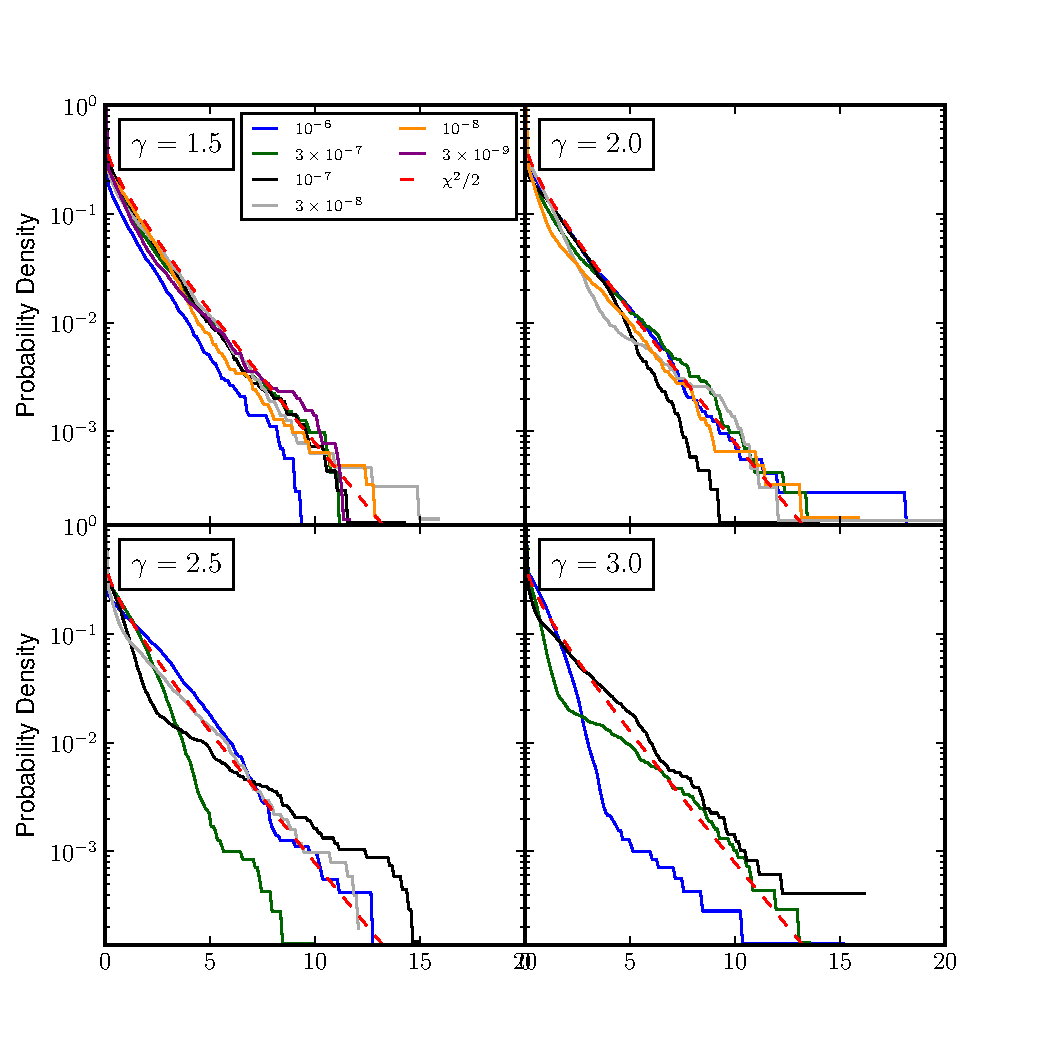
\includegraphics{mc_plots/ts_ext_emin_1000.pdf}
    % this plot came from /u/gl/lande/work/fermi/extended_catalog/monte_carlo/ts_ext/v3/plot.py
    % using data from /nfs/slac/g/ki/ki03/lande/extended_catalog/monte_carlo/ts_ext/v3_emin_1000/merged.hdf5
    \end{center}
    \caption{
    \todo[inline]{Shorten this caption}
    The results of the Monte Carlo simulation described in section
    \ref{monte_carlo_validation} testing the null distribution of
    the likelihood ratio test for extension.  The $x$ axis of this
    plot is \tsext and the $y$ axis is the cumulative density for
    \tsext that was found by testing simulated point sources of
    various spectral models for extension. The four plots represent
    different spectral indices (for $\gamma$ of 1, 2, 2.5, and 3).
    The different colored lines represent different fluxes which were
    chosen to span a representative range of values. The dashed
    red line is the cumulative density function of $\chi^2(\ts)/2$ which is
    suggested by Wilks' theorem as the theoretical distribution these
    curves should should follow.  Overall, it should be noted that there
    is a surprisingly good agreement between the Monte Carlo study and
    the theoeretical distribution. And for most spectral parameters, the
    Monte Carlo curve lies to the left of the theoretical curve, which
    would imply that using Wilks' Theorem as the null distribution would
    conservativly underestimate the signifcance of a source detection. In
    the rest of the paper, we use this theoretical curve to estimate
    the significance of our source detections.  What is quoted is the
    $>100$ \mev integral flux in measured in units of $\ph/\cm^2/\sec$.
    For each spectral model, more information about the simulations is
    summarized in table~\ref{ts_ext_num_sims}. More
    information about this Monte Carlo analysis is presented in
    section~\ref{monte_carlo_validation}.
    }\label{ts_ext_mc}
  \end{figure}

\clearpage

\begin{figure}
  \begin{center}
    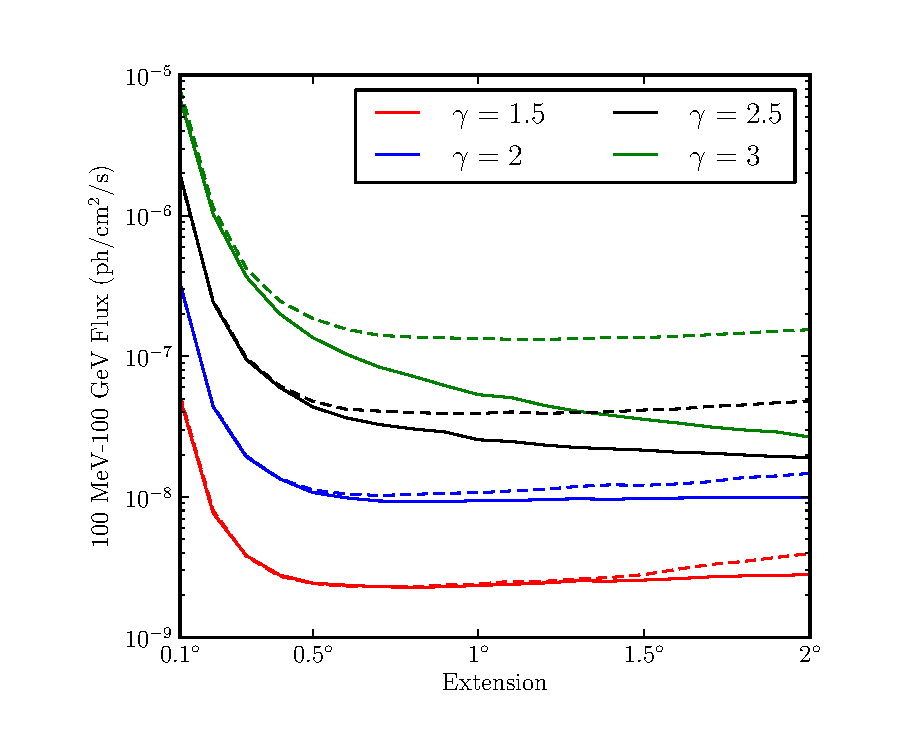
\includegraphics{mc_plots/index_sensitivity.pdf}
    % this plot came from /u/gl/lande/work/fermi/extended_catalog/monte_carlo/sensitivity/v9/plot_vs_index.py
    \end{center}
    \caption{This is the LAT's detection threshold to spatially
    extended sources. The $x$ axis is Monte Carlo extension of a
    simulated uniform disk source and the $y$ axis is the simulated
    source's 100 \mev to 100 \gev photon flux. Each curve represents
    the detection threshold for being able to spatially resolve an
    extended source (when $\langle\tsext\rangle=25$).  
    All sources have an assumed power-law spectrum and the different
    colors are for sources of different simulated spectral indices.
    The dashed line shows simulations using photons with energy between 
    100 \mev and 100 \gev while the solid lien shows simulations
    using photons with energy between 1 \gev and 100 \gev.
    The detection threshold is for a one year simulation against a Sreekumar-like
    isotropic background (\cite{sreekumar_isotropic}).
    This plot shows that our threshold is best for sources that are
    about $1\deg$ large. It also shows that for sources that are neither
    very large nor very soft, our sensitivity is not significantly
    improved using photons with energy between 100 \mev and 1 \gev.  More information
    about this plot is presented in section~\ref{extension_sensitivity}.
    }\label{index_sensitivity}
  \end{figure}

\clearpage

\begin{figure}
  \begin{center}
    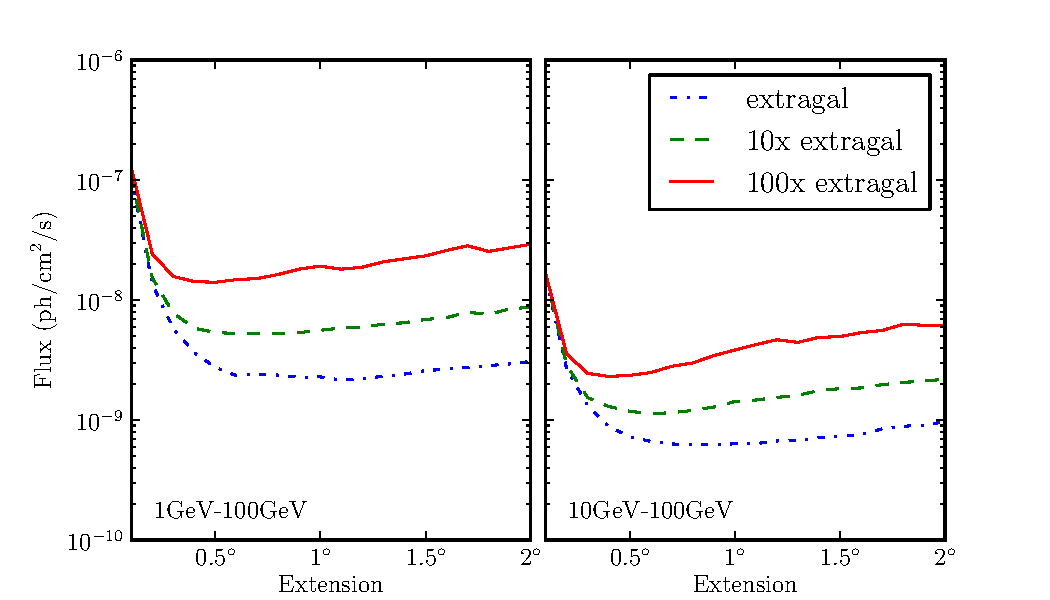
\includegraphics{mc_plots/diff_factor_sensitivity.pdf}
    % this plot came from /u/gl/lande/work/fermi/extended_catalog/monte_carlo/sensitivity/v9/plot_vs_diff_factor.py
    \end{center}
    \caption{
    \todo[inline]{Add Caption}
    }\label{diff_factor_sensitivity}
  \end{figure}

  \begin{figure}
    \begin{center}
      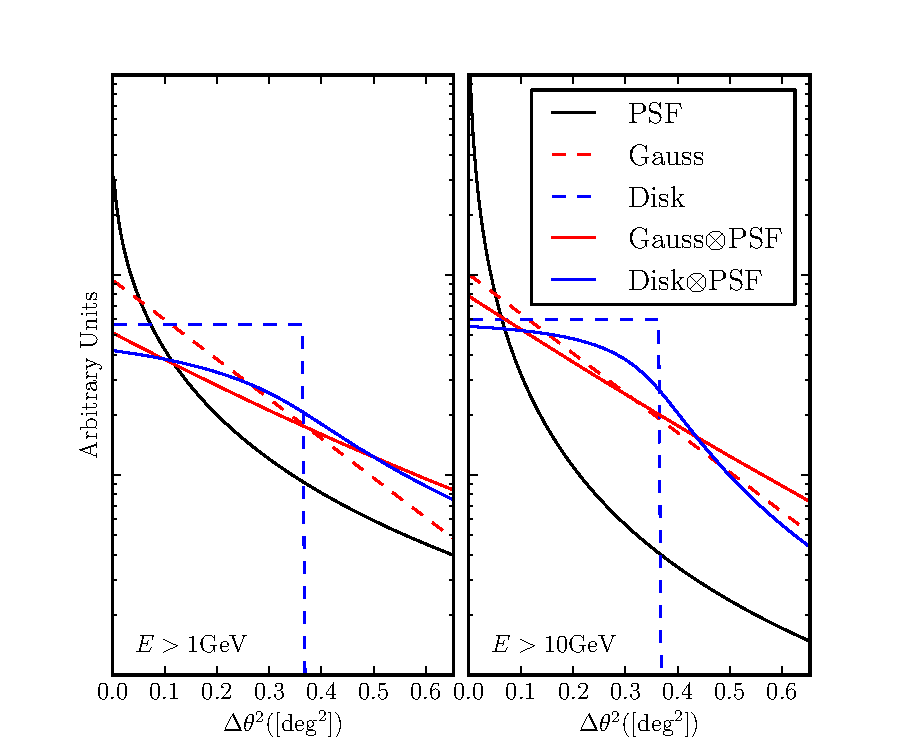
\includegraphics{mc_plots/compare_disk_gauss.pdf}
      % this plot came from /u/gl/lande/work/fermi/extended_catalog/2FGL/plots_for_paper/compare_disk_gauss/v2/compare_disk_gauss.pdf
    \end{center}
    \caption{
    This plot demonstrates that different spatial models when smoothed
    out by the PSF look very similar.  The $y$ axis is the log of the
    intensity and the $x$ axis is $\theta^2$.  The black line is the
    PSF that would be observed for a power-law source of spectral index
    two. The dashed red line is the probability density of a Gaussian
    of width $\rsixeight=0.5\deg$. A Gaussian on this plot is just a
    straight line.  The dashed blue line is the probability density for
    a uniform disk of width $\rsixeight=0.5\deg$.  Finally, the solid
    red and blue lines show the convolution of the Gaussian and uniform
    disk respectively with the PSF.  The left plot shows the analysis
    with an energy range from 1 \gev to 100 \gev whereas the right plot
    shows the analysis with an energy range from 10 \gev to 100 \gev.
    }\label{compare_disk_gauss}
  \end{figure}

  \begin{figure}
    \begin{center}
      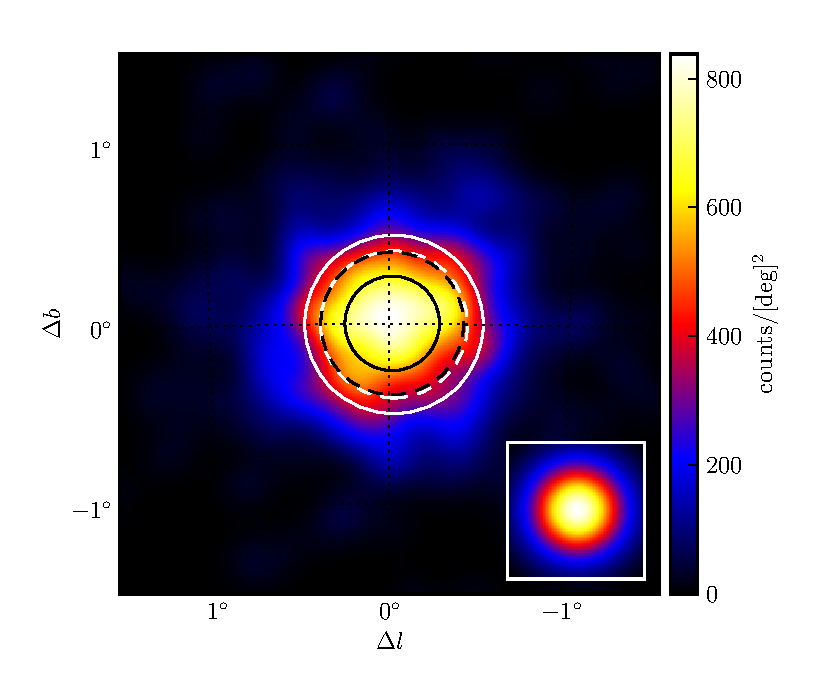
\includegraphics{mc_plots/compare_r68.pdf}
      % this plot came from /u/gl/lande/work/fermi/extended_catalog/2FGL/plots_for_paper/compare_r68/v2/plot.py
      \end{center}
      \caption{A plot of the smoothed counts for a simulated uniform
        disk extended source in the energy range from 1 \gev to 100 \gev.
        The source has a size $\sigma=0.5\deg$, an integral flux between
        1 \gev and 100 \gev of $3\times 10^{-8}\ph/\cm^2/\sec$, and
        a spectral index 2.  The smoothed counts from a point source
        with the same spectrum are shown in the bottom right inset.
        This source was fit with both a uniform disk and a Gaussian
        spatial model.  The white circle represents the fit size $\sigma$
        fitting with the disk hypothesis.  The black circle is the fit
        $\sigma$ fitting with the Gaussian hypothesis.  The dashed white
        and black circles are the fit \rsixeight defined in section
        \ref{compare_source_size} for the disk and Gaussian hypothesis
        respectively.  This plot shows that fitting the same source with
        different spatial shapes can lead to very different values of
        $\sigma$. On the other hand, the different shapes have a good
        agreement about the 68\% containment radius \rsixeight.
      }\label{compare_r68}
    \end{figure}


\begin{figure}
  \begin{center}
  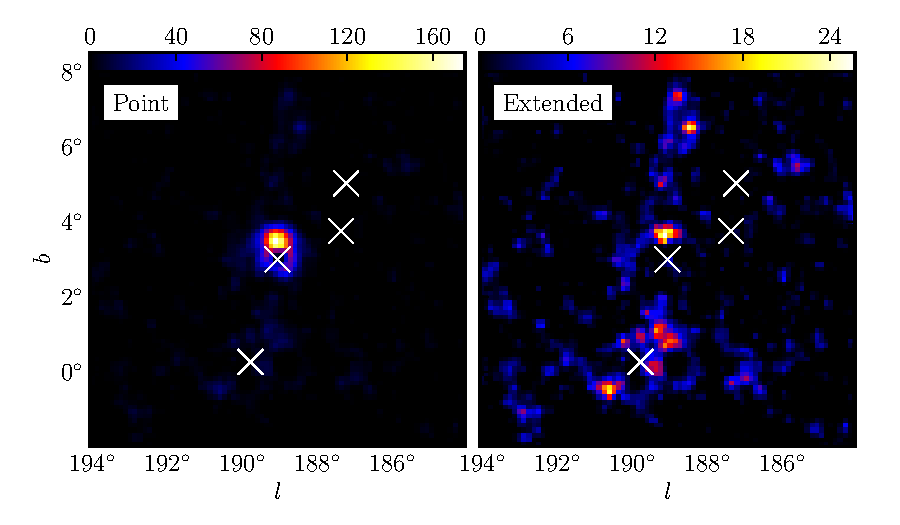
\includegraphics{ic443_plots/res_tsmap_ic443.pdf}
  % plot from /u/gl/lande/work/fermi/extended_catalog/2FGL/plots_for_paper/res_tsmap_ic443/v1

  \caption{An example residual test statistic map generated for the
  supernova remnant IC443 using photons with energy between 1 \gev and
  100 \gev.  The top plot is the residual TS map fitting IC443
  as a point source and the bottom plot is the residual TS map fitting
  IC443 as an extended source. The crosses in the plot represent all of
  the sources fit in the region. Since there is a residual TS greater
  than 160 fitting with the point hypothesis, it is clear that a point
  source is not a good fit to the region. On the other hand,
  the residual TS fitting as an extended source is much lower, showing
  that IC443 is better fit by an extended source. These plots were generated
  for all extended source candidates to help validate the analysis.}
  \label{res_tsmaps}
  \end{center}
\end{figure}

\clearpage
\begin{figure}
  \begin{center}
    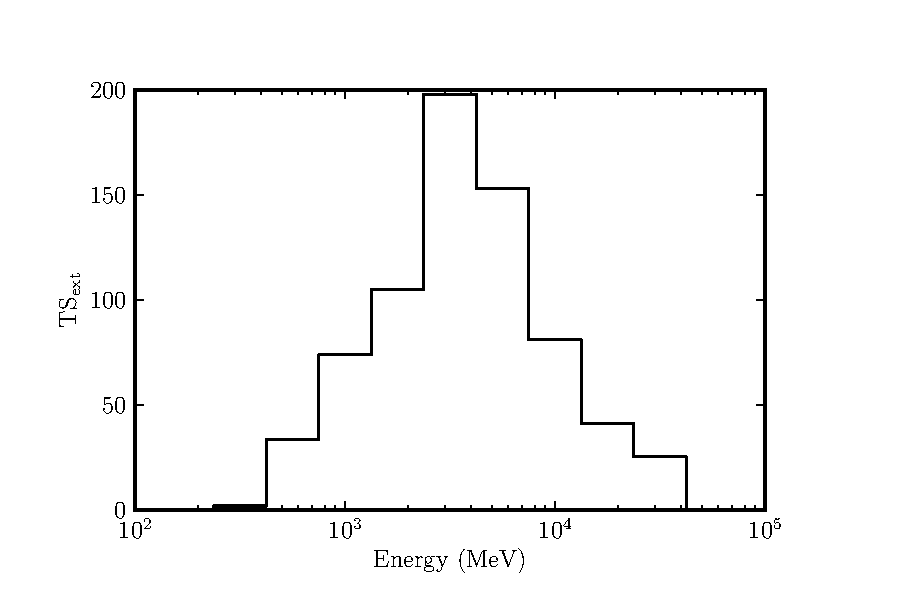
\includegraphics{ic443_plots/ic443_ts_ext_vs_energy.pdf}
    % taken from /u/gl/lande/work/fermi/extended_catalog/2FGL/plots_for_paper/ts_ext_vs_energy/v1/ts_ext_vs_energy.py
    \caption{
    The plot shows \tsext for 12 uniform log(energy) bins between 100
    \mev and 100 \gev for the SNR IC443. IC443 has a spectral index
    ~2.4 (table~\ref{known_extended_sources}) which is typical of
    extended sources.  This plot shows that there is little gain in
    sensitivity in the data with energy below 1 \gev.  For this reason,
    this paper restricts its analysis to energies above 1 \gev.
    }
    \label{ts_ext_vs_energy}
  \end{center}
\end{figure}

\clearpage
\begin{figure}
  \begin{center}
    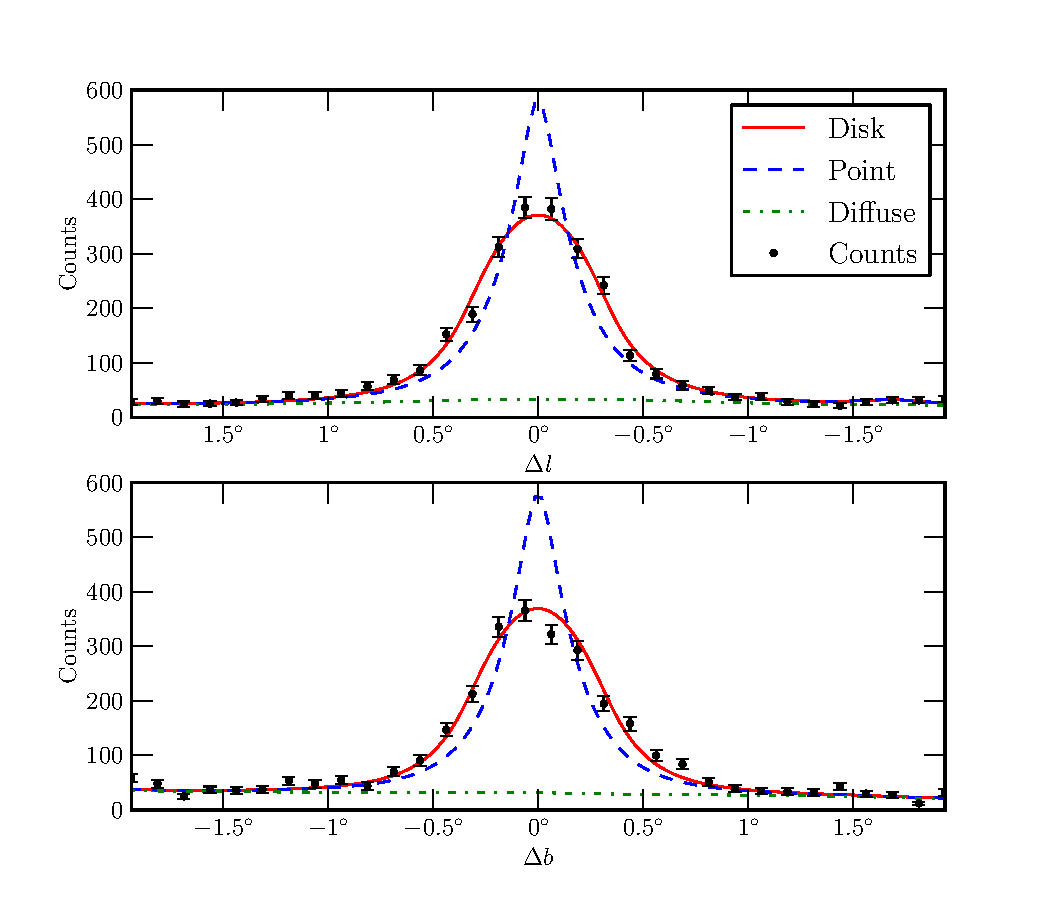
\includegraphics{ic443_plots/ic443_counts_slice.pdf}
    % taken from /u/gl/lande/work/fermi/extended_catalog/2FGL/plots_for_paper/counts_slice_ic443/v1/ic443_counts_slice.pdf
    \caption{
    \todo[inline]{Describe that best for looking at overall diffuse emission and visually assesing quality of the fit.}
    }
    \label{counts_slice}
  \end{center}
\end{figure}

\clearpage
\begin{figure}
  \begin{center}
    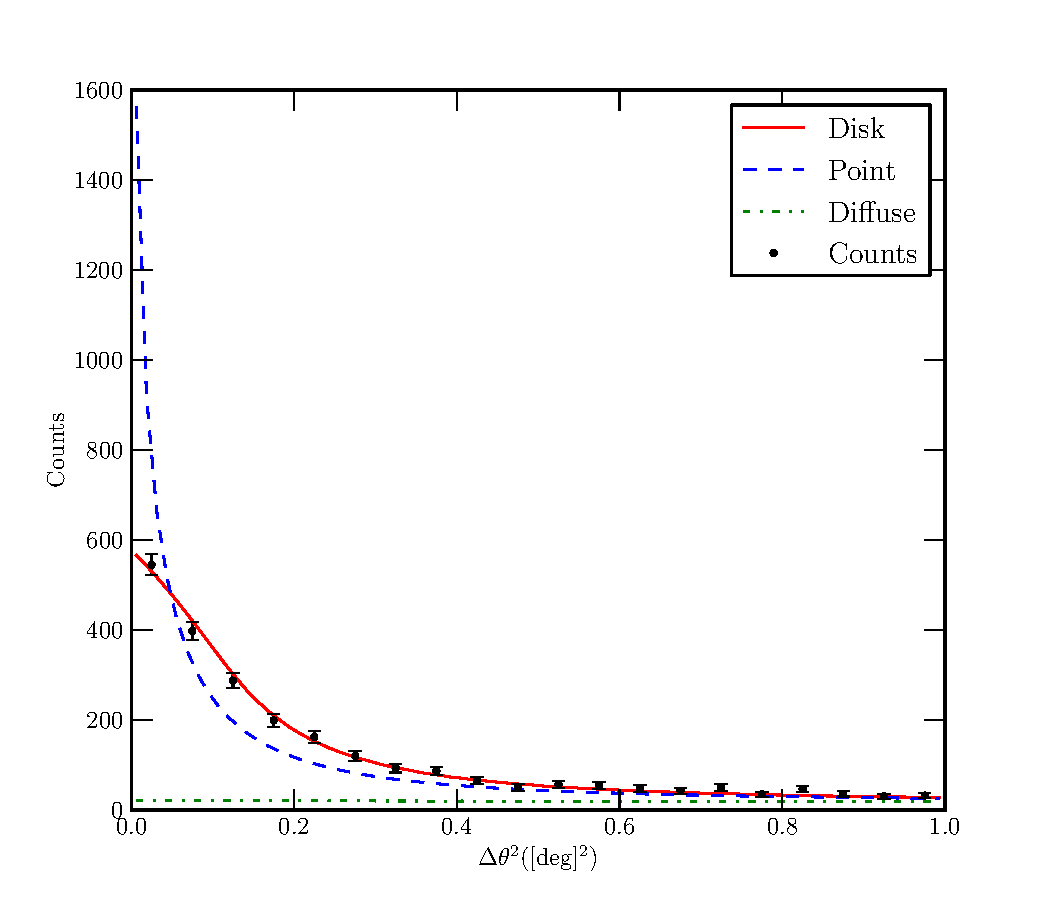
\includegraphics{ic443_plots/ic443_radial_integral.pdf}
    % taken from /u/gl/lande/work/fermi/extended_catalog/2FGL/plots_for_paper/radial_integral_ic443/v1/ic443_radial_integral.pdf
    \caption{The radial integral of the counts and the model predicted counts.
    \todo[inline]{Add more text about why this is useful}
    }
    \label{radial_profile}
  \end{center}
\end{figure}

\clearpage
\begin{figure}
  \begin{center}
    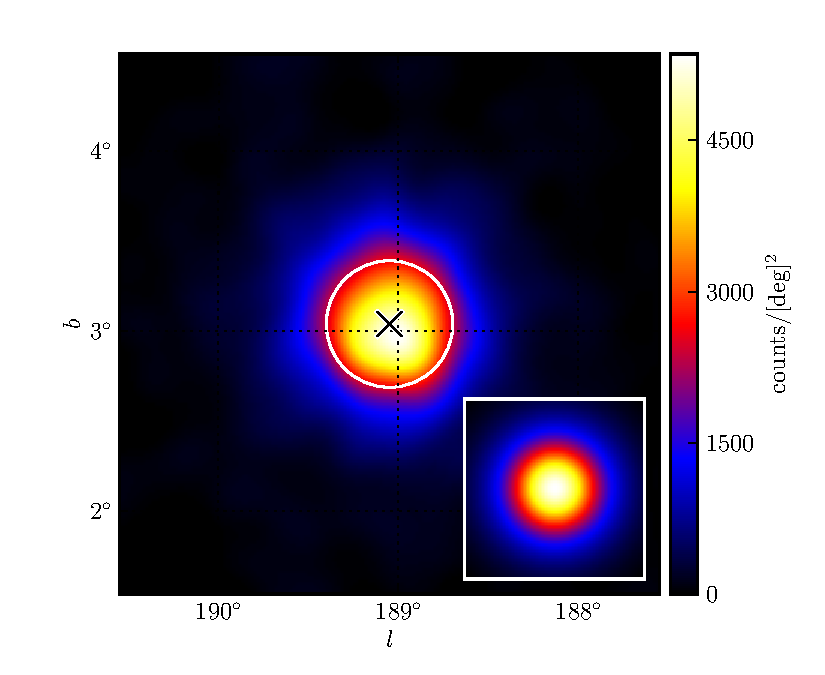
\includegraphics{ic443_plots/ic443_smoothed_counts.pdf}
    % taken from /u/gl/lande/work/fermi/extended_catalog/2FGL/plots_for_paper/smoothed_counts_ic443/v1
    \caption{Smoothed counts. Galactic and isotoropic as well as earth albedo background were subtracted.
    \todo[inline]{describe that this is IC443 using (front? or back? or both?) photons.}
    }
    \label{smoothed_counts}
  \end{center}
\end{figure}

\clearpage
\begin{figure}
  \begin{center}
    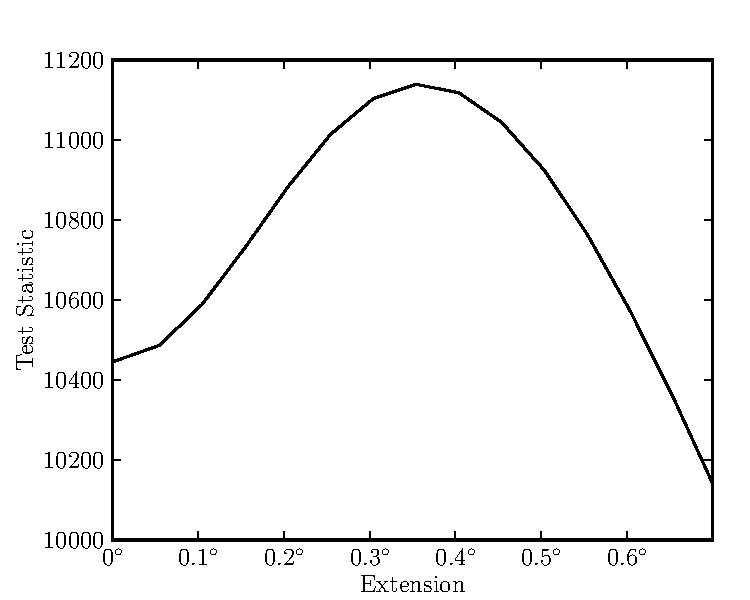
\includegraphics{ic443_plots/profile_ic443.pdf}
    % taken from /u/gl/lande/work/fermi/extended_catalog/2FGL/plots_for_paper/extension_profile_ic443/v1/profile_ic443.pdf
    \caption{
    A plot of the overall change in Test Statistic when varying the
    extension of the extended SNR IC443.  As is discussed in section
    \ref{extension_error}, the error on the extension of a source is
    calculated by varying the extension away from its best fit value until
    the log likelihood has changed by an amount 1/2.  These profiles are
    generated for all extended source candidates. They plot is useful
    to make sure the fitter is not stuck in a local minimum and to make
    sure the profile is reasonably parabolic.
    }
    \label{extension_profile}
  \end{center}
\end{figure}


\clearpage
\begin{figure}
  \begin{center}
    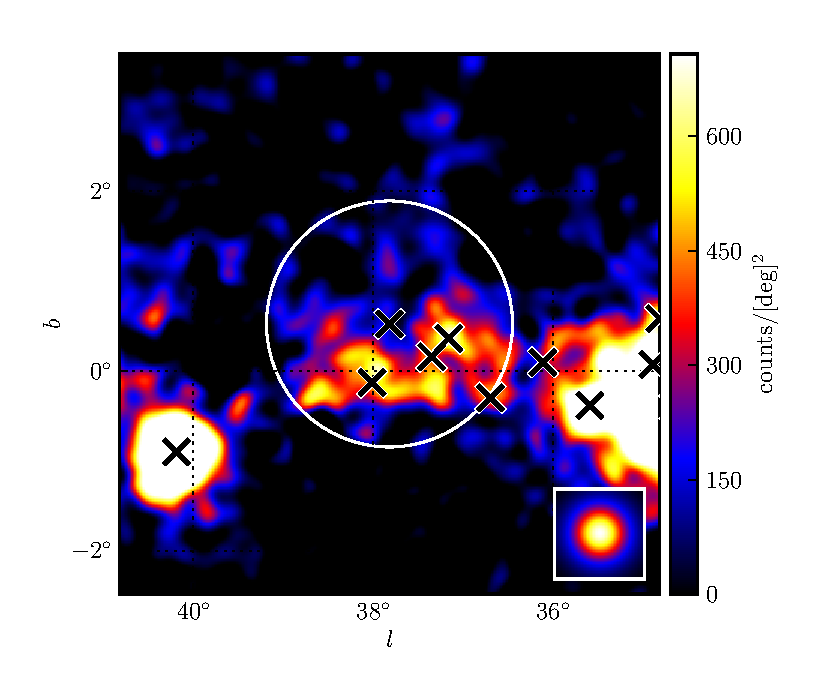
\includegraphics{source_plots/example_bad_fit.pdf}
    % taken from /u/gl/lande/work/fermi/extended_catalog/2FGL/plots_for_paper/example_bad_fit/v2
    \caption{Example bad Fit: P72Y3047
    \todo[inline]{Describe how this is a bad fit}
    }
    \label{example_bad_fit}
  \end{center}
\end{figure}


\clearpage
\begin{sidewaystable}
    \begin{centering}
      \begin{tabular}{r|rrrrrrrrrr}
        \hline
        \hline
        Name                 &          \glon &          \glat &                    $\sigma$ &       TS &   $\tsext$ &      Major &      Minor &    Pos Ang &      Flux ($10^{-9}$) &                 Index \\
        \hline
        \multicolumn{11}{c}{$E > 1\gev$} \\
        \hline
        SMC                  &     302.87\deg &     -44.65\deg & $  1.59\deg \pm   0.15\deg$ &     93.1 &       51.2 &  0.173\deg &  0.129\deg &   41.9\deg & $    3.0 \pm     0.4$ & $   2.42 \pm    0.16$ \\
        LMC                  &     278.58\deg &     -32.82\deg & $  2.26\deg \pm   0.09\deg$ &    384.2 &      304.4 &  0.096\deg &  0.071\deg &  -35.5\deg & $   12.9 \pm     0.7$ & $   2.42 \pm    0.08$ \\
        IC443                &     189.05\deg &       3.04\deg & $  0.35\deg \pm   0.01\deg$ &  10765.3 &      535.3 &  0.006\deg &  0.006\deg &   84.0\deg & $   65.2 \pm     1.2$ & $   2.23 \pm    0.02$ \\
        W28                  &       6.51\deg &      -0.29\deg & $  0.39\deg \pm   0.02\deg$ &   1231.3 &       92.1 &  0.014\deg &  0.013\deg &   30.4\deg & $   55.9 \pm     1.8$ & $   2.65 \pm    0.03$ \\
        W30                  &       8.61\deg &      -0.20\deg & $  0.36\deg \pm   0.04\deg$ &    458.1 &       66.0 &  0.020\deg &  0.018\deg &   14.1\deg & $   30.0 \pm     1.8$ & $   2.58 \pm    0.06$ \\
        W44                  &      34.68\deg &      -0.42\deg & $  0.34\deg \pm   0.02\deg$ &   1387.6 &      111.3 &  0.009\deg &  0.009\deg &  -39.4\deg & $   74.7 \pm     1.0$ & $   2.67 \pm    0.01$ \\
        W51C                 &      49.12\deg &      -0.44\deg & $  0.28\deg \pm   0.02\deg$ &   2174.7 &       87.6 &  0.010\deg &  0.010\deg &   59.4\deg & $   41.6 \pm     1.3$ & $   2.38 \pm    0.04$ \\
        \hline
        \multicolumn{11}{c}{$E > 10\gev$} \\
        \hline
        HESS J1825-137       &      17.58\deg &      -0.46\deg & $  0.64\deg \pm   0.08\deg$ &     85.6 &       62.5 &  0.050\deg &  0.045\deg &   33.6\deg & $    1.8 \pm     0.3$ & $   1.75 \pm    0.20$ \\
        MSH 15-52            &     320.39\deg &      -1.22\deg & $  0.20\deg \pm   0.06\deg$ &     73.7 &        9.5 &  0.033\deg &  0.032\deg &    3.9\deg & $    0.6 \pm     0.1$ & $   2.32 \pm    0.23$ \\

      \end{tabular}
      \caption{The fit results for the already known extended sources that
      were found by our analysis. The top results were found using an
      energy range between 1 \gev and 100 \gev.  The lower analysis
      was done using photons between 10 \gev and 100 \gev.  The quoted
      flux is in units of $10^{-9}\ph/\cm^2/\sec$ and is the flux in the
      fit energy range (either 1 \gev to 100 \gev or 10 \gev to 100 \gev).
      All sources were fit using a uniform disk spatial template. The
      localization and extension were found using \pointlike while the
      TS and spectral values were calculated using \gtlike.  The TS value
      was computed using the assumed disk morphology and \tsext compares
      is the increase in \ts fitting the source with an extended spatial
      model instead of a point model.  \glon and \glat are respectively
      the galactic longitude and galactic latitude of the source and
      $\sigma$ is the edge of the uniform disk spatial model that was fit
      to the source.  The Centaurus A Lobes, the Cygnus Loop, and Vela
      X were not found to be extended by this too. The
      reasons for this are discussed in section~\ref{validate_known}.
      }
      \label{known_extended_sources}
    \end{centering}
\end{sidewaystable}

\clearpage
\begin{figure}
  \begin{center}
    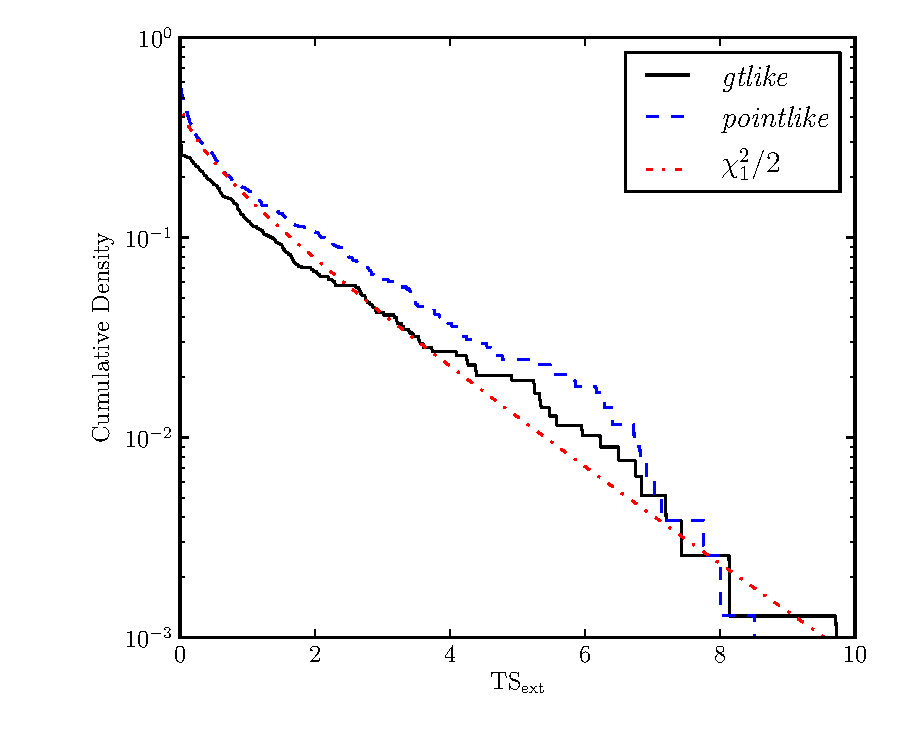
\includegraphics{source_plots/agn.pdf}
    % this plot came from /u/gl/lande/work/fermi/extended_catalog/2FGL/agn/v2/agn.py
    \end{center}
    \caption{
    \todo[inline]{Add Caption.
    Note about how \tsext for AGN calculated with pointlike}
    }\label{agn_ts_ext}
  \end{figure}


  % 1FGL J1628.6-2419c - P72Y2516         - 2FGL J1627.0-2425c
  % 1FGL J1554.0-5345c - P72Y2405         - 2FGL J1554.4-5317c
  % 1FGL J0823.3-4248  - P72Y1212         - 2FGL J0823.0-4246
  % 1FGL J1613.6-5100c - P72Y2473         - 2FGL J1615.2-5138
  % 1FGL J1632.9-4802c - P72Y2540         - 2FGL J1632.4-4753c
  % 1FGL J2020.0+4049  - P72Y3281         - 2FGL J2021.5+4026
  % 1FGL J1837.5-0659c - P72Y2974         - 2FGL J1837.3-0700c
  % N/A                - P72Y1287         - 2FGL J0851.7-4635


\clearpage
\begin{sidewaystable}
  \begin{centering}
    \begin{tabular}{r|rrrrrrrrrr}
      \hline
      \hline
      Name                 &          \glon &          \glat &                    $\sigma$ &       TS &   $\tsext$ &      Major &      Minor &    Pos Ang &      Flux ($10^{-9}$) &                 Index \\
      \hline
      \multicolumn{11}{c}{$E > 1\gev$} \\
      \hline
      2FGL J1627.0-2425c   &     353.08\deg &      16.80\deg & $  0.41\deg \pm   0.05\deg$ &    139.2 &       28.9 &  0.042\deg &  0.036\deg &   54.4\deg & $    6.3 \pm     0.6$ & $   2.50 \pm    0.14$ \\
      2FGL J1554.4-5317c   &     328.13\deg &       0.26\deg & $  0.49\deg \pm   0.04\deg$ &    148.8 &       77.6 &  0.046\deg &  0.041\deg &   55.3\deg & $   16.2 \pm     1.5$ & $   2.31 \pm    0.11$ \\
      2FGL J0823.0-4246    &     260.31\deg &      -3.28\deg & $  0.37\deg \pm   0.03\deg$ &    314.6 &       49.2 &  0.026\deg &  0.023\deg &    5.0\deg & $    8.3 \pm     0.3$ & $   2.18 \pm    0.02$ \\
      \hline
      \multicolumn{11}{c}{$E > 10\gev$} \\
      \hline
      2FGL J1615.2-5138          &     331.74\deg &      -0.58\deg & $  0.52\deg \pm   0.04\deg$ &     75.3 &       45.2 &  0.071\deg &  0.049\deg &  -21.9\deg & $    1.3 \pm     0.2$ & $   1.75 \pm    0.25$ \\
      2FGL J1632.4-4753c         &     336.52\deg &       0.06\deg & $  0.65\deg \pm   0.03\deg$ &    173.0 &       95.3 &  0.041\deg &  0.037\deg &    5.3\deg & $    2.9 \pm     0.2$ & $   2.28 \pm    0.08$ \\
      2FGL J2021.5+4026          &      78.33\deg &       2.22\deg & $  0.71\deg \pm   0.04\deg$ &    245.7 &      151.7 &  0.047\deg &  0.038\deg &    4.3\deg & $    2.1 \pm     0.2$ & $   2.36 \pm    0.18$ \\
      2FGL J1837.3-0700c         &      25.09\deg &       0.13\deg & $  0.35\deg \pm   0.07\deg$ &     47.3 &       20.6 &  0.076\deg &  0.063\deg &   -7.7\deg & $    1.0 \pm     0.2$ & $   1.59 \pm    0.30$ \\
      2FGL J0851.7-4635          &     266.29\deg &      -1.43\deg & $  1.15\deg \pm   0.08\deg$ &    119.6 &       90.9 &  0.080\deg &  0.065\deg &   54.6\deg & $    1.3 \pm     0.2$ & $   1.76 \pm    0.18$ \\
      \hline
    \end{tabular}
    \caption{The 8 new source candidates found by the
    extended source search. 3 new extended sources were found searching looking at photons with energies 1 \gev and
    5 new candidates were found looking at photons with energies above 10 \gev.
    The columns in this table have the same definition as table~\ref{known_extended_sources}.
    More information about these sources can be found in section~\ref{new_ext_srcs_section}
    }
    \label{new_ext_srcs_table}
  \end{centering}
\end{sidewaystable}


\clearpage
\begin{sidewaystable}
    \begin{centering}
      \begin{tabular}{r|rr|rrrr|rrrr}
        \hline
        \hline
        Name                 &     \tsinc &     \tsext &      $\glon_1$ &      $\glat_1$ & $\text{Flux}_1$ ($10^{-9}$) &   $\text{Index}_1$ &      $\glon_2$ &      $\glat_2$ & $\text{Flux}_1$ ($10^{-9}$) &  $\text{Index}_2$ \\
        \hline
        \multicolumn{11}{c}{$E > 1\gev$} \\
        \hline
        2FGL J1627.0-2425c   &       23.8 &       28.9 &     353.04\deg &      16.96\deg & $       3.5 \pm        0.6$ & $  2.7 \pm   0.3$  &     353.14\deg &      16.50\deg & $       2.0 \pm        0.5$ & $  2.4 \pm   0.3$ \\
        2FGL J1554.4-5317c   &       48.6 &       77.6 &     328.31\deg &       0.31\deg & $      10.0 \pm        1.2$ & $  2.7 \pm   0.2$  &     328.28\deg &      -0.06\deg & $       1.0 \pm        0.7$ & $  1.6 \pm   0.4$ \\
        2FGL J0823.0-4246    &       22.2 &       49.2 &     260.59\deg &      -3.26\deg & $       2.0 \pm        0.5$ & $  1.9 \pm   0.2$  &     260.24\deg &      -3.20\deg & $       5.3 \pm        0.6$ & $  2.4 \pm   0.1$ \\
        \hline
        \multicolumn{11}{c}{$E > 10\gev$} \\
        \hline
        2FGL J1615.2-5138    &       34.3 &       45.2 &     331.77\deg &      -0.35\deg & $       0.3 \pm        0.1$ & $  1.1 \pm   0.5$  &     331.51\deg &      -0.83\deg & $       0.4 \pm        0.1$ & $  2.1 \pm   0.5$ \\
        2FGL J1632.4-4753c   &       24.8 &       95.3 &     336.16\deg &       0.34\deg & $       0.7 \pm        0.1$ & $  2.0 \pm   0.4$  &     336.72\deg &      -0.06\deg & $       0.7 \pm        0.1$ & $  3.1 \pm   0.5$ \\
        2FGL J2021.5+4026    &       34.5 &      151.7 &      78.08\deg &       2.53\deg & $       0.4 \pm        0.1$ & $  2.0 \pm   0.5$  &      78.45\deg &       2.54\deg & $       0.5 \pm        0.1$ & $  1.9 \pm   0.4$ \\
        2FGL J1837.3-0700c   &       15.4 &       20.6 &      25.06\deg &       0.24\deg & $       0.3 \pm        0.1$ & $  1.1 \pm   0.6$  &      25.08\deg &      -0.05\deg & $       0.4 \pm        0.1$ & $  1.9 \pm   0.6$ \\
        2FGL J0851.7-4635    &       32.5 &       90.9 &     267.16\deg &      -1.60\deg & $       0.2 \pm        0.1$ & $  1.9 \pm   0.4$  &     266.43\deg &      -1.39\deg & $       0.2 \pm        0.1$ & $  1.5 \pm   0.5$ \\
        \hline
      \end{tabular}
      \label{dual_localization_results}
      \caption{For the new extended source candidates in
      table~\ref{new_ext_srcs_table}, we describe the results
      of the dual localization procedure described in
      section~\ref{dual_localization_method}. Here, the extended
      source candidate is not fit as an extended source but instead
      fit as two point sources.  The dual localization is performed
      with \pointlike and results in the best fit position of the two
      sources $(\glon_1,\glat_1)$ and $(\glon_2,\glat_2)$.  The change
      in likelihood and spectral values are then computed using \gtlike
      with the best fit positions found by \pointlike.  \tsinc is the
      increase in TS fitting the region as two sources compared to
      fitting compared to fitting a single point source and is computed
      using \gtlike with the best fit positions taken from \pointlike.
      It can be directly compared to \tsext, which is taken from table~\ref{new_ext_srcs_table}.  For all of our candidates, $\tsext > \tsinc$
      which shows that an extended source fits the source better than two
      point sources.  As in table~\ref{known_extended_sources}, flux is
      measured in units of $10^{-9}\ph/\cm^2/\sec$ and is the integral
      flux between 1 \gev (10 \gev) and 100 \gev for the sources found
      using photons above 1 \gev (10 \gev).}
    \end{centering}
  \end{sidewaystable}


  \clearpage
  \begin{sidewaystable}
    \begin{centering}
      \begin{tabular}{r|rrrrrrrr}
        \hline
        \hline
        Name                 &     $\ts_\pointlike$ &        $\ts_\gtlike$ &           $\ts_\alt$ &          \tsextpointlike &           \tsextgtlike &            \tsextalt &                    $\sigma$ &               $\sigma_\alt$ \\
        \hline
        \multicolumn{9}{c}{$E > 1\gev$} \\
        \hline
        2FGL J1627.0-2425c   &                155.0 &                139.2 &                103.8 &                     38.5 &                   28.9 &                 22.5 & $  0.41\deg \pm   0.05\deg$ & $  0.38\deg \pm   0.04\deg$ \\
        2FGL J1554.4-5317c   &                108.4 &                148.8 &                138.4 &                     25.7 &                   77.6 &                 40.6 & $  0.49\deg \pm   0.04\deg$ & $  0.51\deg \pm   0.04\deg$ \\
        2FGL J0823.0-4246    &                329.5 &                314.6 &                345.6 &                     60.4 &                   49.2 &                 51.5 & $  0.37\deg \pm   0.03\deg$ & $  0.38\deg \pm   0.03\deg$ \\
        \hline
        \multicolumn{9}{c}{$E > 10\gev$} \\
        \hline
        2FGL J1615.2-5138    &                 74.7 &                 75.3 &                 88.7 &                     43.7 &                   45.2 &                 50.0 & $  0.52\deg \pm   0.04\deg$ & $  0.53\deg \pm   0.03\deg$ \\
        2FGL J1632.4-4753c   &                173.9 &                173.0 &                157.7 &                     97.9 &                   95.3 &                 93.6 & $  0.65\deg \pm   0.03\deg$ & $  0.66\deg \pm   0.03\deg$ \\
        2FGL J2021.5+4026    &                244.9 &                245.7 &                264.3 &                    152.8 &                  151.7 &                162.9 & $  0.71\deg \pm   0.04\deg$ & $  0.71\deg \pm   0.03\deg$ \\
        2FGL J1837.3-0700c   &                 43.4 &                 47.3 &                 39.0 &                     17.4 &                   20.6 &                 17.7 & $  0.35\deg \pm   0.07\deg$ & $  0.34\deg \pm   0.06\deg$ \\
        2FGL J0851.7-4635    &                117.1 &                119.6 &                124.7 &                     86.1 &                   90.9 &                 95.0 & $  1.15\deg \pm   0.08\deg$ & $  1.16\deg \pm   0.08\deg$ \\
        \hline
      \end{tabular}
      \label{alt_diff_model_results}
      \caption{
      This table shows a comparison of the \ts values gotten using \gtlike and \pointlike.
      It also compares the fit values using the standard diffuse model and using the alternate
      diffuse model described in section~\ref{alt_diff_model_description}.
      $\ts_\pointlike$ is the \ts of the source fit with the extended hypothesis using \pointlike
      whereas $\ts_\gtlike$ is the same quantity using the same model but fitting with \gtlike.
      There is very good agreement between the two methods.
      }
    \end{centering}
  \end{sidewaystable}


\begin{figure}
  \begin{center}
    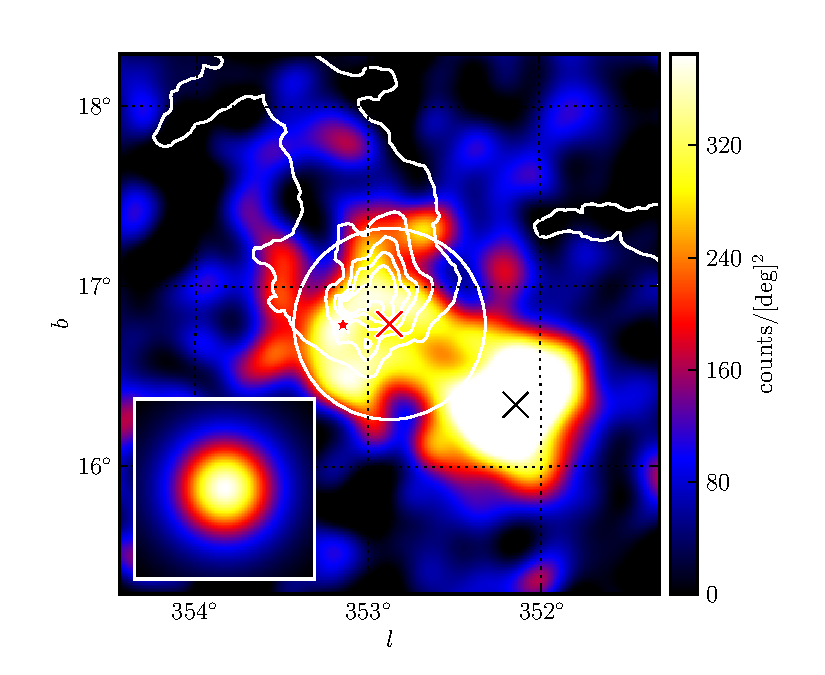
\includegraphics[type=pdf,ext=.pdf,read=.pdf]{source_plots/source_1FGL_J1628.6-2419c}
  \end{center}
  % this plot came from 
  % /u/gl/lande/work/fermi/extended_catalog/2FGL/plots_for_paper/source_plots/1FGL_J1628.6-2419c/v2/run.py
  \caption{1FGL J1628.6-2419c. In the opiucus region=most likeliy a molecular cloud.
  %P72Y2516.
  \todo[inline]{Add description of this source.
  Note the bright nearby source
  which would be in the lower right of the image at $l,b=352.14\deg,16.34\deg$.
  $\ts=460$, source is P72Y2510. What is this source?}
  }\label{1FGL_J1628.6-2419c}
\end{figure}

\begin{figure}
  \begin{center}
    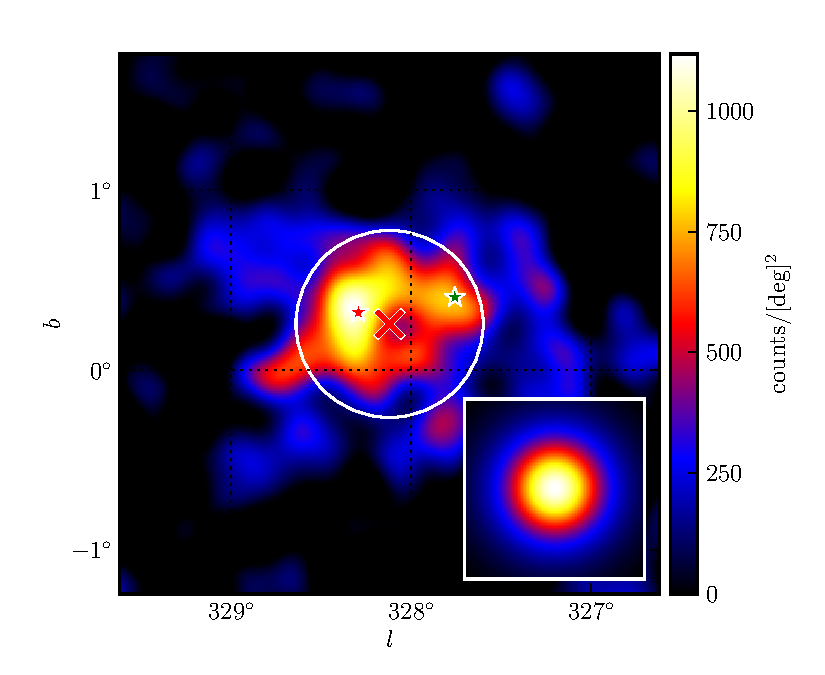
\includegraphics[type=pdf,ext=.pdf,read=.pdf]{source_plots/source_1FGL_J1554.0-5345c}
  \end{center}
  % this plot came from 
  % /u/gl/lande/work/fermi/extended_catalog/2FGL/plots_for_paper/source_plots/1FGL_J1554.0-5345c/v2/source_1FGL_J1554.0-5345c.pdf
  \caption{1FGL J1554.0-5345c. 
  %P72Y2405. 
  \todo[inline]{Describe this source/the fit.Unidentified source likely diffuse emission.}
  }
  \label{1FGL_J1554.0-5345c}
\end{figure}

\begin{figure}
  \begin{center}
    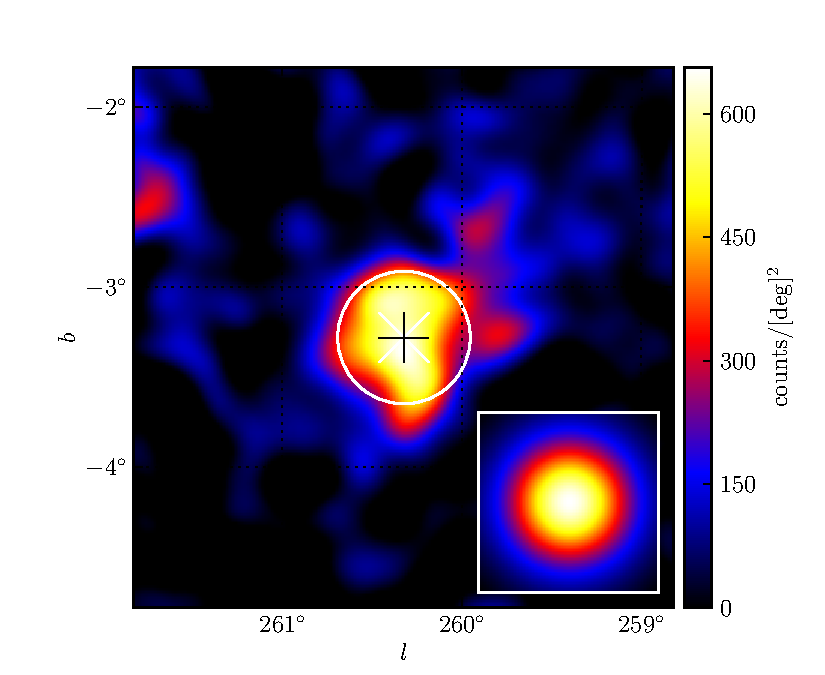
\includegraphics[type=pdf,ext=.pdf,read=.pdf]{source_plots/source_1FGL_J0823.3-4248}
  \end{center}
  % this plot came from 
  % /u/gl/lande/work/fermi/extended_catalog/2FGL/plots_for_paper/source_plots/1FGL_J0823.3-4248/v2/source_1FGL_J0823.3-4248.pdf
  \caption{1FGL J0823.3-4248. P72Y1212. Coincident with Puppis A SNR.
  %P72Y1212.
  \todo[inline]{
  Describe this soruce better.
  Describe nearby source Vela.
  At position $l,b=263.55\deg,-2.79\deg$ is over 3 degrees away,
  Spills into the image at left.}
  \todo[inline]{Describe this source better. Add in Contour}
  }\label{1FGL_J0823.3-4248}
\end{figure}

\begin{figure}
  \begin{center}
    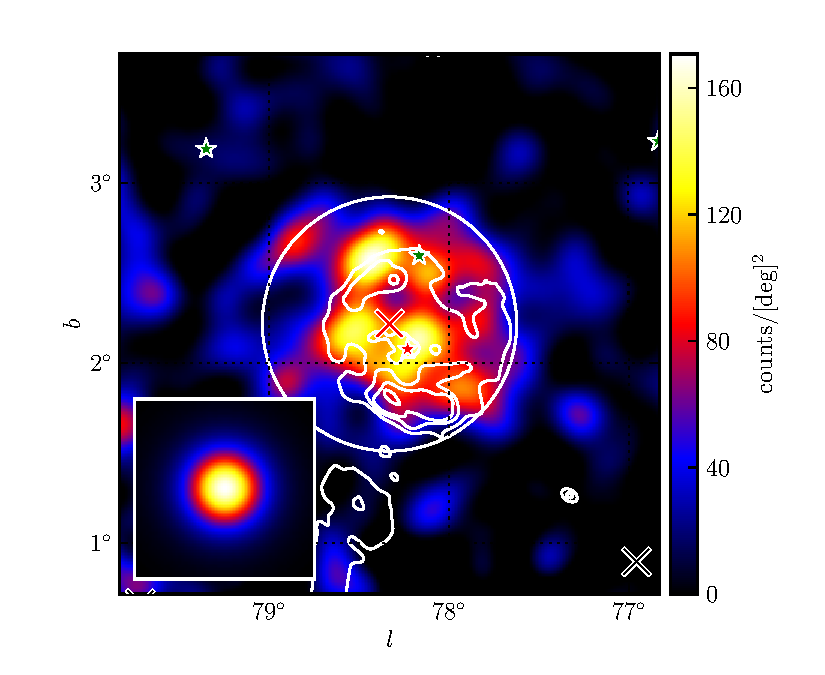
\includegraphics[type=pdf,ext=.pdf,read=.pdf]{source_plots/source_Gamma_Cygni}
  \end{center}
  % this plot came from 
  % /u/gl/lande/work/fermi/extended_catalog/2FGL/plots_for_paper/source_plots/Gamma_Cygni/v2/source_Gamma_Cygni.pdf
  \caption{
  Gamma Cygni. P72Y3281
  \todo[inline]{Describe this source better. Add in Contour}
  }\label{Gamma_Cygni}
\end{figure}

\begin{figure}
  \begin{center}
    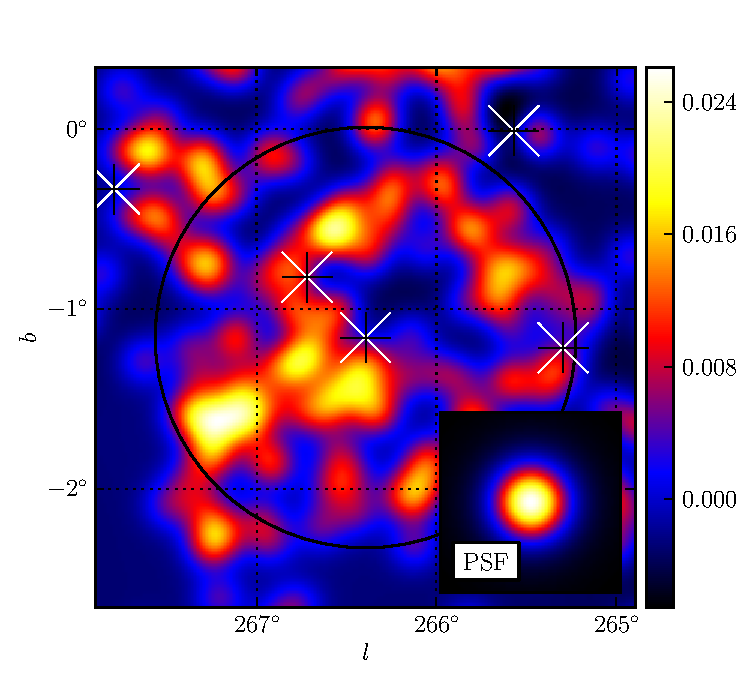
\includegraphics[type=pdf,ext=.pdf,read=.pdf]{source_plots/source_Vela_Jr}
  \end{center}
  % this plot came from 
  % /u/gl/lande/work/fermi/extended_catalog/2FGL/plots_for_paper/source_plots/Vela_Jr/v2/source_Vela_Jr.pdf
  \caption{Vela Jr. P72Y1287. Using $E>10\gev$. 
  \todo[inline]{Note that sourceis con with a $0.25\deg$ gaussian which is different than other plots.}
  \todo[inline]{Describe this source better. Add in Contour}
  }\label{Vela_Jr}
\end{figure}

\begin{figure}
  \begin{center}
    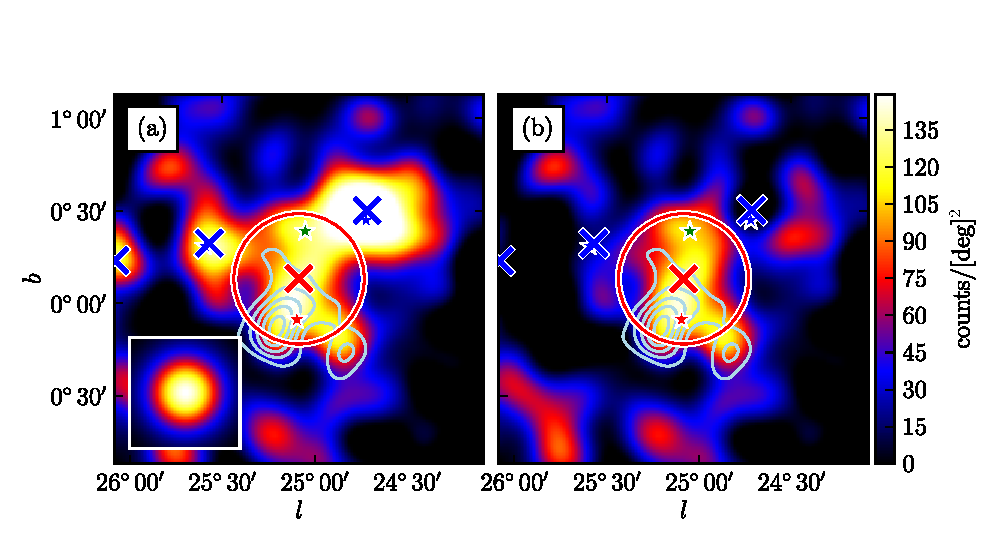
\includegraphics[type=pdf,ext=.pdf,read=.pdf]{source_plots/source_1FGL_J1837.5-0659c}
  \end{center}
  % this plot came from 
  % /u/gl/lande/work/fermi/extended_catalog/2FGL/plots_for_paper/source_plots/1FGL_J1837.5-0659c/v2/source_1FGL_J1837.5-0659c.pdf
  \caption{1FGL J1837.5-0659c. P72Y2974
  \todo[inline]{Describe this source better. Add in Contour}
  \todo[inline]{Note about why the top right source was not found to
  be extended b/c the scale is cut.}
  }\label{1FGL_J1837.5-0659c}
\end{figure}


\begin{figure}
  \begin{center}
    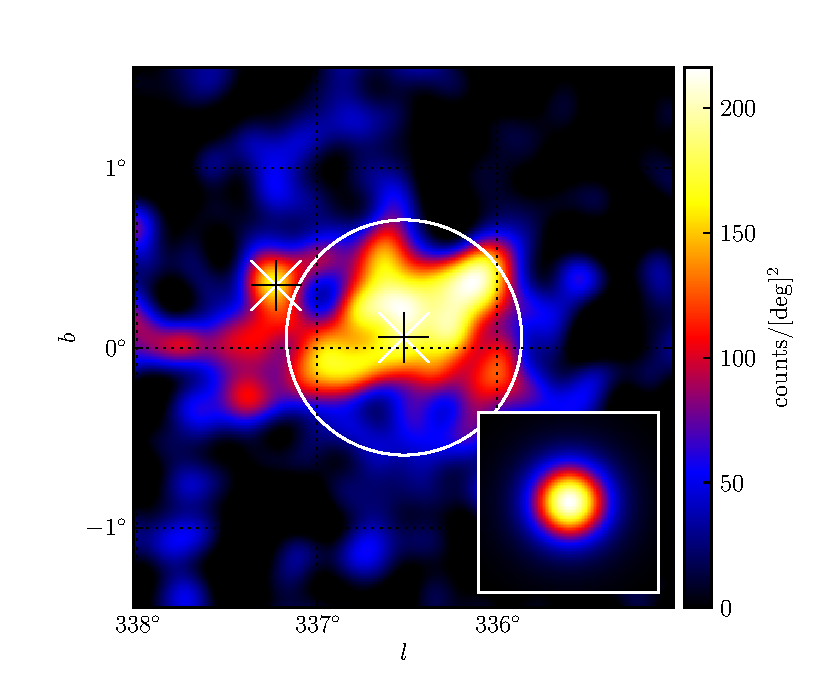
\includegraphics[type=pdf,ext=.pdf,read=.pdf]{source_plots/source_1FGL_J1632.9-4802c}
  \end{center}
  % this plot came from 
  % /u/gl/lande/work/fermi/extended_catalog/2FGL/plots_for_paper/source_plots/1FGL_J1632.9-4802c/v2/source_1FGL_J1632.9-4802c.pdf
  \caption{1FGL J1632.9-4802c. P72Y2540
  \todo[inline]{Describe this source better. Add in Contour}
  }\label{1FGL_J1632.9-4802c}
\end{figure}


\begin{figure}
  \begin{center}
    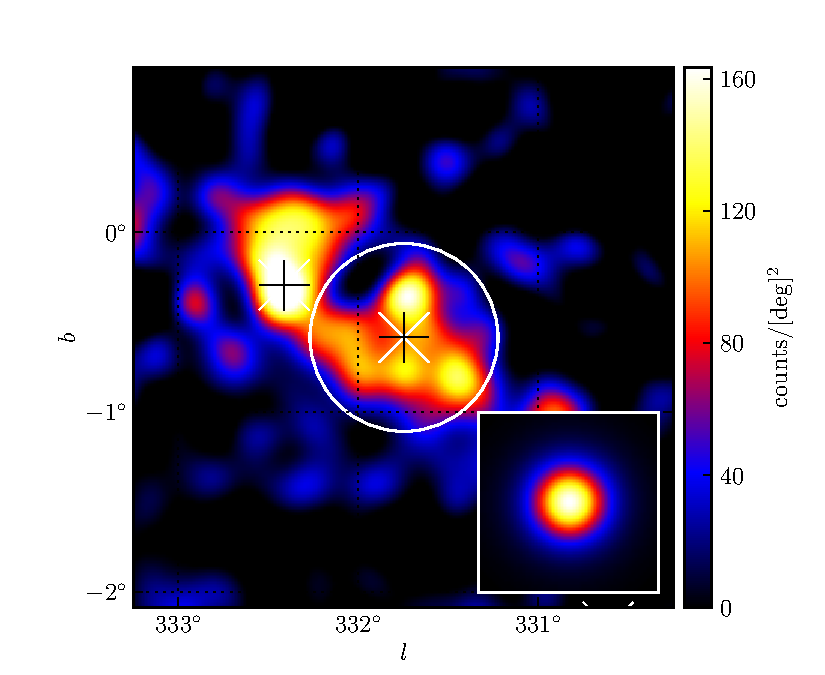
\includegraphics[type=pdf,ext=.pdf,read=.pdf]{source_plots/source_1FGL_J1613.6-5100c}
  \end{center}
  % this plot came from 
  % /u/gl/lande/work/fermi/extended_catalog/2FGL/plots_for_paper/source_plots/1FGL_J1613.6-5100c/v2/source_1FGL_J1613.6-5100c.pdf
  \caption{
  1FGL J1613.6-5100c . P72Y2473
  \todo[inline]{Describe this source better. Add in Contour}
  }\label{1FGL_J1613.6-5100c}
\end{figure}


\end{document}
